\documentclass[conference]{IEEEtran}
%\documentclass{sig-alternate-2013}
%\documentclass{llncs}
\usepackage{makeidx}
\usepackage{tabularx,colortbl}
\usepackage[dvipsnames]{xcolor}
%\usepackage{flushend}
\usepackage{cite}
%\usepackage{authblk}
\usepackage{amsmath}
%\usepackage{amsthm}
\usepackage{amssymb}
\usepackage{bm}
\usepackage{epsfig}
\usepackage{stmaryrd}
\usepackage{url}
\usepackage{multirow}
\usepackage{latexsym}
\usepackage{graphics}
\usepackage{multicol}
\usepackage{dblfloatfix}
%\usepackage{lipsum}
\usepackage{graphicx}
\usepackage{enumitem}
\usepackage{comment}
\usepackage{longtable}
\usepackage{supertabular}
\usepackage{times}
\usepackage{listings}
\usepackage{subfigure}
\usepackage{color}
\usepackage{balance}
\usepackage{xspace}
\usepackage[ruled, vlined, linesnumbered]{algorithm2e}
\usepackage[autostyle]{csquotes}
\usepackage[]{algorithm2e}
%\usepackage{textcomp}
%\usepackage[font=large]{caption}
\widowpenalty10000




%\theoremstyle{Definition}
%\newtheorem{definition}{Definition}
%%%
%\theoremstyle{Theorem}
%\newtheorem{theorem}{Theorem}


%\newcommand{\definition}{\noindent \textbf{Definition} \citation{}}
%\newcommand{\theorem}{\noindent \textbf{Theorem} \citation{}}
%\newcommand{\lemma}{\noindent \textbf{Lemma} \citation{}}

%\newdef{lemma}{Lemma}
%\newdef{definition}{Definition}
%\newdef{theorem}{Theorem}
%\newdef{corollary}{Corollary}
%\newdef{note}{Note}
%\newdef{axiom}{Axiom}
\newcommand{\mkeyword}[1]{\mbox{\texttt{#1}}}
\DeclareMathOperator{\kuop}{uop}
\DeclareMathOperator{\kbop}{bop}
\DeclareMathOperator{\kite}{ite}
\DeclareMathOperator{\kpre}{pre}
\DeclareMathOperator{\dom}{dom}
\DeclareMathOperator{\ktrue}{true}
\DeclareMathOperator{\kfalse}{false}
\DeclareMathOperator{\kselect}{select}
\DeclareMathOperator{\ran}{range}
\newcommand{\lbb}{[\![}
\newcommand{\rbb}{]\!]}
\newcommand{\expr}{\phi}
\newcommand{\exprS}{\Phi}
\newcommand{\mats}[1]{\textcolor{red}{#1}}
\newcommand{\janet}[1]{\textcolor{blue}{#1}}
\newcommand{\darren}[1]{\textcolor{green}{#1}}
\newcommand{\danielle}[1]{\textcolor{orange}{#1}}

\sloppypar



\begin{document}

\definecolor{gold}{rgb}{0.90,.66,0}
\definecolor{dgreen}{rgb}{0,0.6,0}
\newcommand{\stateequiv}{\equiv_{s}}
\newcommand{\traceequiv}{\equiv_{\sigma}}
\newcommand{\ta}{\text{TA}}
\newcommand{\cta}{\text{TA$_{C}$}}
\newcommand{\tta}{\text{TA$_{T}$}}
\newcommand{\ucalg}{\texttt{\small{IVC\_UC}}}
\newcommand{\ucbfalg}{\texttt{\small{IVC\_UCBF}}}


\title{Safety Annex for the 
\\Architecture Analysis and Design Language
%\thanks{This work is funded by NASA under contract NLL16AA09B.}
}

%
%\author{Danielle Stewart %\inst{1}
%\and Jing (Janet) Liu% \inst{2}
%\and Michael W. Whalen\inst{1}
%\and Darren Cofer %\inst{2}
%\and Mats Heimdahl %\inst{1}
%\and Michael Peterson %\inst{3}}
%\institute{University of Minnesota\\Department of Computer
%Science and Engineering\\
%\email{dkstewar, whalen, heimdahl}@cs.umn.edu
%\and
%Collins Aerospace\\
%%Advanced Technology Center
%Trusted Systems - Engineering and Technology
%\\
%\email{Jing.Liu, Darren.Cofer}@collins.com
%\and
%Collins Aerospace\\
%%Commercial Systems 
%Flight Controls Safety Engineering - Avionics\\
%\email{Michael.Peterson}@collins.com
%}

%\numberofauthors{2}
%\author{
%\alignauthor
%Andrew Gacek, John Backes,\\ Darren Cofer, Konrad Slind\\
%       \affaddr{Rockwell Collins}\\
%       \affaddr{Advanced Technology Center}\\
%       \email{first.last@rockwellcollins.com}
%\alignauthor
%Mike Whalen\\
%       \affaddr{University of Minnesota}\\
%       \affaddr{Computer Science Department}\\
%       \email{whalen@cs.umn.edu}
%}



\author{
    \IEEEauthorblockN{Danielle Stewart\IEEEauthorrefmark{1}, Jing (Janet) Liu\IEEEauthorrefmark{2}, Darren Cofer\IEEEauthorrefmark{2}, Mats Heimdahl\IEEEauthorrefmark{1}, Michael W. Whalen\IEEEauthorrefmark{1}, Michael Peterson\IEEEauthorrefmark{2}}
    \IEEEauthorblockA{\IEEEauthorrefmark{1}University of Minnesota, Department of Computer Science
    \\\{dkstewar, heimdahl, mwwhalen\}@umn.edu}
    \IEEEauthorblockA{\IEEEauthorrefmark{2}Collins Aerospace
    \\\{jing.liu, darren.cofer, michael.peterson\}@collins.com}
}

\maketitle

\begin{abstract}

Model-based development tools are increasingly being used 
for system-level development of safety-critical systems. Architectural 
and behavioral models  provide important information 
that can be leveraged to improve the system
safety analysis process. Model-based design artifacts 
produced in early stage development activities can be used to perform system safety analysis,
reducing costs, and providing accurate results throughout
the system life-cycle.  In this paper we describe an extension 
to the Architecture Analysis and Design Language (AADL) that 
supports modeling of system behavior under failure conditions. This 
\emph{Safety Annex} enables the independent modeling of component 
failures and allows safety engineers to weave various types of 
fault behavior into the nominal system model. The accompanying tool support 
uses model checking to propagate errors from their source to
 their effect on top-level safety properties without the need to add 
separate propagation specifications. Our tools are also able to 
compute minimal cutsets for these errors to produce faults trees 
familiar to safety engineers and certification authorities.  
We describe the Safety Annex, illustrate its use with a representative 
example, and discuss and demonstrate the tool support enabling an 
analyst to investigate the system behavior under failure conditions.	
	
\end{abstract}

%\keywords{Model-based systems engineering, fault analysis, safety engineering}

\section{Introduction}
\label{sec:intro}

%Mats' intro
System safety analysis is crucial in the development life cycle of critical systems to ensure adequate safety as well as demonstrate compliance with applicable standards. A prerequisite for any safety analysis is a thorough understanding of the system architecture and the behavior of its components; safety engineers use this understanding to explore the system behavior to ensure safe operation, assess the effect of failures on the overall safety objectives, and construct the accompanying safety analysis artifacts. Developing adequate understanding, especially for software components, is a difficult and time consuming endeavor. Given the increase in model-based development in critical systems~\cite{Joshi05:Dasc,CAV2015:BoCiGrMa,info17:HaLuHo,5979344,Gudemann:2010:FQQ:1909626.1909813}, leveraging the resultant models in the safety analysis process holds great promise in terms of analysis accuracy as well as efficiency.

In this paper we describe the \emph{Safety Annex} for the system engineering language AADL (Architecture Analysis and Design Language), a SAE Standard modeling language for Model-Based Systems Engineering (MBSE)~\cite{AADL_Standard}. The Safety Annex allows an analyst to model the failure modes of components and then ``weave'' these failure modes together with the original models developed as part of MBSE. The safety analyst can then leverage the merged behavioral models to propagate %failures
errors through the system to investigate their effect on the safety requirements. %(implicit %failure
%error propagation). 

%Darren
In previous work, we have extended AADL to include formal \emph{assume-guarantee} contracts describing the behavior of systems and components \cite{NFM2012:CoGaMiWhLaLu}.  These contracts describe the nominal behavior of the system, and can be used to formally verify system requirements through compositional reasoning applied to the each hierarchical layer in the AADL model.  The Safety Annex builds on this approach by adding language constructs for specifying the possible behaviors of systems and components in the presence of faults.  When a fault is triggered in the model, its nominal contract is replaced by the specified failure contract and the resulting impact on the system can be analyzed using a model checker.  This focus on the behavior of the system in the presence of failures is fundamentally different from the capabilities provided by the existing AADL Error Model Annex \cite{EMV2}, and enables powerful new approaches to system safety analysis.  

Determining how %faults
errors propagate through software components is currently a costly and time-consuming element of the safety analysis process. 
\begin{comment} 
The use of behavioral contracts to capture the implicit %fault
error propagation characteristics of software component is a significant benefit for safety analysts.  
In addition, the annex allows modeling of explicit %failure 
error propagation that is not captured through the behavioral models, for example, the effect of a single electrical failure on multiple software components or the effect hardware failure (e.g., an explosion) on multiple behaviorally unrelated components. 
\end{comment}
The use of behavioral contracts to capture the %implicit %fault
error propagation characteristics of software component without the need to add separate propagation specifications (\emph{implicit} error propagation) is a significant benefit for safety analysts.  
In addition, the annex allows modeling of %explicit %failure 
dependent faults that are not captured through the behavioral models (\emph{explicit} error propagation),
%error propagation that is not captured through the behavioral models, 
for example, the effect of a single electrical failure on multiple software components or the effect hardware failure (e.g., an explosion) on multiple behaviorally unrelated components. 
Furthermore, we will describe the tool support enabling engineers to investigate the correctness of the nominal system behavior (where no failures have occurred) as well as the system's resilience to component failures. We illustrate the work with an  %substantial 
example drawn from the civil aviation domain.

Our work can be viewed as a continuation of work conducted by Joshi et al.~where they explored model-based safety analysis techniques defined over Simulink/Stateflow~\cite{MathWorks} models~\cite{Joshi05:SafeComp,Joshi07:Hase,Joshi05:Dasc,DBLP:conf/cav/BozzanoCPJKPRT15}. Our current work extends this work to provide new modeling and analysis capabilities.  For example, the Safety Annex supports compositional verification and exploration of the nominal system behavior as well as the system's behavior under failure conditions. 
Related work includes the AADL Error Annex (EMV2)~\cite{EMV2}, COMPASS~\cite{10.1007/978-3-642-04468-7_15}, and AltaRica~\cite{PROSVIRNOVA2013127,BieberERTS2018}. 
Our approach differs from AADL EMV2 in that we leverage the behavioral modeling for implicit error propagation.  We provide compositional analysis capabilities that are not available in COMPASS.  The Safety Annex  is fully integrated in a model-based development process and environment unlike a stand alone language like AltaRica. 

%The main contributions of this project and the Safety Annex are:
The main contributions of the AADL Safety Annex are:
\begin{itemize}
\renewcommand{\labelitemi}{\textbullet}
		\item close integration of behavioral fault analysis into the {\em Architecture Analysis and Design Language} AADL, which allows close connection between system and safety analysis and system generation from the model,
		\item support for {\em behavioral specification of faults} and their {\em implicit propagation} (both symmetric and asymmetric) through behavioral relationships in the model, in contrast to existing AADL-based annexes (HiP-HOPS~\cite{CHEN201391}, EMV2~\cite{EMV2}) and other related toolsets (COMPASS~\cite{10.1007/978-3-642-04468-7_15}, Cecilia~\cite{bieber2004safety}, etc.),
		\item additional support to capture binding relationships between hardware and software and logical and physical communications, %and
		\item computation of all minimal fault combinations that can cause violation of the safety properties to be compared to qualitative and quantitative objectives as part of the safety assessment process, and
		\item guidance on integration into a traditional safety analysis process.
\end{itemize}

%\janet{add reference and citation to NASA report}


%The remainder of the paper is organized as follows. INSERT WHATEVER IT ENDED UP LOOKING LIKE. 

\begin{comment}
%Danielle's and Janet's intermediate intro

System safety analysis techniques are crucial in the development life cycle of highly integrated/complex aircraft systems and are used to show compliance with certification requirements. A prerequisite of performing any safety assessment of a system design is to understand how the system is intended to work, primarily focusing on the relationship between component outputs and the overall behavior of the system. The safety engineers then use this information to conduct safety analysis, construct the safety analysis artifacts, and compare the analysis results with established safety objectives and safety-related requirements. Acquiring knowledge about the behavior of the software applications hosted in a system and its impact on the overall system behavior is typically a time consuming and involved process.

To help solve this problem, researchers and industry practitioners have turned to the use of models. Models have been shown to be an effective way to help engineers capture, understand and analyze complex systems. Previous work has been done showing the benefits of leveraging the system model in the safety analysis process~\cite{Joshi05:SafeComp,Joshi07:Hase,Joshi05:Dasc,DBLP:conf/cav/BozzanoCPJKPRT15}.

%In order to effectively assist safety engineers to acquire the knowledge on software application behaviors and assess their effects on the overall behavior of the system, the models should allow system designers to capture the expected behaviors of the software application and the expected behavioral propagations among different components/application in the system; and allow safety engineers to leverage the same model provided by system designers, capture failure modes for individual components, and automatically assess the effects to the overall system through the behavioral propagations built in the existing model.

During this safety analysis process, it is important to reason about faults and how faulty component behaviors can impact the overall system behavior. In order to address the problem of understanding the model and complex system, it is advantageous to provide an automated analysis framework that allows for various types of fault definitions, propagations, and modeling options. 

This paper introduces a tool that provides a solution to these problems: the Safety Annex for the system engineering language called Architecture Analysis and Design Language (AADL), a widely used SAE Standard design language for MBSE applications~\cite{AADL_Standard}. Given a system model in AADL and a behavioral model developed in the Assume Guarantee Reasoning Environment (AGREE)~\cite{NFM2012:CoGaMiWhLaLu}, the Safety Annex is a fault modelling tool that utilizes model checking in order to analyze the behavior of a system in the presence of faults. The Safety Annex allows safety engineers to leverage existing models from system development for conducting assessment. 

Throughout this paper we show that the Safety Annex allows both implicit and explicit failure propagation which gives richer fault modeling capabilities than comparable tools. It is also shown how behavioral information regarding the active faults, the component properties and the overall system behavior when faults are active are provided. We demonstrate that the toolset (AADL, AGREE, and Safety Annex) captures behaviors of both the nominal model (absence of faults) and the faulty model in a cleanly separated and yet analyzable fashion. This serves to preserve the system model for the systems engineering process and simultaneously be able to see their combined effect on the system behavior. 


 %Using a Model-Based Safety Analysis (MBSA) approach allows safety engineers to weave a fault model into the entire MBSE process while preserving the separation of a system model and a fault model.


%To help solve this problem, researchers and industry practitioners have turned to Model-based System Engineering (MBSE). Models have been shown to be an effective way to help engineers capture, understand and analyze complex systems. Previous work has been done showing the benefits of leveraging the system model in the safety analysis process~\cite{Joshi05:SafeComp,Joshi07:Hase,Joshi05:Dasc,DBLP:conf/cav/BozzanoCPJKPRT15}. Using a Model-Based Safety Analysis (MBSA) approach allows an analyst \janet{use the term ``safety engineer'' only or both ``safety engineer'' and ``safety analyst''?} to weave a fault model into the entire MBSE process while preserving the separation of a system model and a fault model.
\end{comment}

\iffalse

Throughout the development life cycle of highly-integrated/complex aircraft systems, safety assessment process is a crucial piece in asserting development assurance, and is used to show compliance with certification requirements and meeting a company's internal safety standards. A prerequisite of performing any safety assessment of a system design is to understand how the system is intended to work, primarily focusing on the relationship between component outputs and the overall behavior of the system. The safety engineers then use the acquired understanding to conduct safety analysis, construct the safety analysis artifacts, and compare the analysis results with established safety objectives and safety-related requirements.  

In practice, prior to performing the safety assessment of a system, the safety engineers are often equipped with the domain knowledge about the system, but do not necessarily have detailed knowledge of how the software functions are designed. Acquiring the required knowledge about the behavior and implementation of each software function in a system is typically the most time consuming and involved step in the process.

Industry practitioners have come to realize the benefits and importance of
using models to assist the safety assessment process, such as to better understand system behaviors, communicate with system designers, capture the failure propagations, and manage and analyze more complex systems. And a revision to the Guidelines and Methods for Conducting Safety Assessment Process on Civil Airborne Systems and Equipment~\cite{SAE:ARP4761} to include {\em model based safety analysis} is under way.

%condensed version
%System safety assessment is a crucial process in the development of complex airborne systems to show that the relevant safety requirements are met. Acquiring the required knowledge about how the software functions are intended to work in such systems has shown in practice a very involved and time consuming task. Existing approaches that annotate the system architecture model with failure modes and fault propagations help safety analysts better communicate with system designers and address the complexity of the system. However, knowledge on how the faults propagate through the components still needs to be acquired by safety analysts before such information can be captured in the model. Acquiring the information on fault propagation is still a manual effort.

We think that the following criteria are important for the models to help safety analysts effectively acquire the knowledge about system/software behaviors and capture/analyze failure propagations:

\begin{itemize}
	\item Allow safety engineers to leverage existing models from system development for conducting assessment. %This captures the current state of the system design as it moves through the system development lifecycle, reducing the gap in comprehending the system behavior and transferring the knowledge between the system designers and the safety analysts.
	\item Support capturing behaviors of nominal and faulty behaviors in the system that are cleanly separated, yet analyzable in an integrated fashion to see their combined effect on the system.
	\item Enable safety engineers to inject failures/faults at component level, and assess the effect of behavioral propagation at system level, without needing to acquire the knowledge on the propagation beforehand. 
	\item Allow safety engineers to add failure propagations to the model that may not be behavioral related such as common cause/hardware dependent faults (e.g., common failures such as pipe burst that can propagate through physical systems).
\end{itemize}

%The methodology described in this paper enables safety analysts to specify faults and faulty behaviors at individual components (using the Safety Annex for the Architecture Analysis and Design Language (AADL)). 

%The provided tool support auto weaves the faults into the nominal system model provided by system designers. No additional effort is needed to specify fault propagations as the faulty behavior propagates in the nominal system model the same as the normal behavior. The behavior of the system in the presence of faults are verified using model checking through Assume Guarantee Reasoning Environment (AGREE), and the effects of any triggered fault are manifested in the formal analysis results.

%1. Introduce our approach and it addresses all that
%2. behavioral propagation of failures
%3. We could just describe/split in implicit and explicit fault/failure propagations. E.g., for explicit failure propagation, now we can connect behaviorally unrelated components.
%3. You activate a fault/inject a failure to the system, so it's not fault propagation, but failure propagation

%How we evaluate our work in comparison with others'
%1. There are other approaches support some of them. However, they don't support ...
%What are the related work and why they don't solve the problem:
%Researchers like Anjali have explored ...
%EMV2
%xSAP
%2. What we do is different from XXX because ...
%3. The EMV2 is really talking about failure propagation. They view errors as corrupted states. That lead to certain level of confusion. 
%4. In ARP4754, an error is treated as a source of fault, but a fault can happen without error. An error might lead to a fault. A SW can have errors as software doesn't fail on its own - someone has to put it there

\begin{comment}
%This paper describes a new methodology with tool support for model based safety analysis. It is implemented as a {\em Safety Annex} for the Architecture Analysis and Design Language (AADL). The Safety Annex provides the ability to describe faults and faulty component behaviors in AADL models. In contrast to previous AADL-based approaches, the Safety Annex leverages a formal description of the nominal system behavior to propagate faults in the system. This approach ensures consistency with the rest of the system development process and simplifies the work of safety engineers. The language for describing faults is extensible and allows safety engineers to weave various types of faults into the nominal system model. The Safety Annex supports the injection of faults into component level outputs, and the resulting behavior of the system can be analyzed using model checking through the Assume-Guarantee Reasoning Environment (AGREE).

System safety analysis techniques are well-established and are a required activity in the development of safety-critical systems. Model-based systems engineering (MBSE) methods and tools based on formal methods now permit system-level requirements to be specified and analyzed early in the development process~\cite{NFM2012:CoGaMiWhLaLu,CAV2015:BoCiGrMa}. While model-based development methods are widely used in the aerospace industry, they are only recently being applied to system safety analysis.  

%How can we leverage these model-based methods and tools to perform safety analysis based on models of the system architecture and initial functional decomposition? Can these design models be integrated into the safety analysis process to help guarantee accurate and consistent results?
%Seeking solutions to these questions are especially important as the amount of safety-critical hardware and software in various domains has drastically increased due to the demand for greater autonomy, capability, and connectedness.

In this paper, we describe a {\em Safety Annex} for the Architecture Analysis and Design Language (AADL)~\cite{FeilerModelBasedEngineering2012} that provides the ability to reason about faults and faulty component behaviors in AADL models. In the Safety Annex approach, we use formal assume-guarantee contracts to define the nominal behavior of system components. The nominal model is then verified using the Assume Guarantee Reasoning Environment (AGREE)~\cite{NFM2012:CoGaMiWhLaLu}. The Safety Annex  provides a way to weave faults into the nominal system model and analyze the behavior of the system in the presence of faults. The Safety Annex also provides a library of common fault node definitions that is customizable to the needs of system and safety engineers. Our approach adapts the work of Joshi et. al in
~\cite{Joshi05:Dasc} to the AADL modeling language, and provides a domain specific language for the kinds of analysis performed manually in previous work~\cite{Stewart17:IMBSA}.  %More information on the approach is available in~\cite{Stewart17:IMBSA}, and the tool and relevant documentation can be found at: \small \url{https://github.com/loonwerks/AMASE/}. \normalsize

%There are other tools purpose-built for safety analysis, including AltaRica~\cite{PROSVIRNOVA2013127}, smartIFlow~\cite{info8010007} and xSAP~\cite{DBLP:conf/tacas/BittnerBCCGGMMZ16}. These notations are separate from the system development model. Other tools extend existing system models, such as HiP-HOPS~\cite{CHEN201391} and the AADL Error Model Annex, Version 2 (EMV2)~\cite{EMV2}. EMV2 uses enumeration of faults in each component and explicit propagation of faulty behavior to perform safety analysis. The required propagation relationships must be manually added to the system model and can become complex, leading to potential omissions and inconsistencies.

The Safety Annex supports model checking and quantitative reasoning by attaching behavioral faults to components and then using the normal behavioral propagation and proof mechanisms built into the AGREE AADL annex. This allows users to reason about the evolution of faults over time, and produce counterexamples demonstrating how component faults lead to system failures. It can serve as the shared model to capture system design and safety-relevant information, and produce both qualitative and quantitative description of the causal relationship between faults/failures and system safety requirements.
%
Thus, the contributions of the Safety Annex and this paper are:
\begin{itemize}
\item Close integration of behavioral fault analysis into the {\em architectural design language} AADL, which allows close connection between system and safety analysis and system generation from the model,
\item support for {\em behavioral specification of faults} and their {\em implicit propagation} through behavioral relationships in the model, in contrast to existing AADL-based annexes (HiP-HOPS, EMV2) and other related toolsets (COMPASS, Cecilia, etc.),
\item additional support to capture binding relationships between hardware and software and logical and physical communications, and
\item guidance on integration into a traditional safety analysis process.
\end{itemize}
%\mike{What are our contributions?}
\end{comment}

\fi

\section{Preliminaries}
\label{sec:prelims}
One of our goals is to transition the tools we have developed into use by the safety engineers who perform safety assessment of avionics products. Therefore, we need to understand how the tools and the models will fit into the existing safety assessment and certification process.
\subsection{Safety Assessment Process}
\label{subsec:process}

%ARP4754A, the Guidelines for Development of Civil Aircraft and Systems~\cite{SAE:ARP4754A}, has been recognized by the Federal Aviation Administration (FAA) as 
%an ``acceptable method for establishing a development assurance process''~\cite{AC:20-174}. It provides guidance on applying development assurance at each hierarchical level throughout the development life cycle of highly-integrated/complex aircraft systems.

ARP4754A, the Guidelines for Development of Civil Aircraft and Systems~\cite{SAE:ARP4754A}, provides guidance on applying development assurance at each hierarchical level throughout the development life cycle of highly-integrated/complex aircraft systems, and has been recognized by the Federal Aviation Administration (FAA) as an acceptable method to establish the assurance process.

%Figure~\ref{fig:arp4754a_process} from [ref. ARP4754A] demonstrates the ARP4754A process flow.

The safety assessment process is a starting point at each hierarchical level of the development life cycle, and is tightly coupled with the system development and verification processes. It is used to show compliance with certification requirements, and for meeting a company's internal safety standards. ARP4761, the Guidelines and Methods for Conducting Safety Assessment Process on Civil Airborne Systems and Equipment~\cite{SAE:ARP4761},  identifies a systematic means to show compliance. The guidelines presented in ARP4761 include industry accepted safety assessment processes (Functional Hazard Assessment (FHA), Preliminary System Safety Assessment (PSSA), and System Safety Assessment (SSA)), and safety analysis methods to conduct the safety assessment, 
such as Fault Tree Analysis (FTA), Failure Modes and Effect Analysis (FMEA), and Common Cause Analysis (CCA).

A prerequisite of performing the safety assessment of a system design is to understand how the system is intended to work, primarily focusing on the integrity of the outputs and the availability of the system. The safety engineers then use the acquired understanding to conduct safety analysis, construct the safety analysis artifacts, and compare the analysis results with established safety objectives and safety-related requirements. 

%In practice, prior to performing the safety assessment of a system, the safety engineers are often equipped with the domain knowledge about the system, but do not necessarily have detailed knowledge of the current system is implemented. Acquiring the required knowledge about the behavior and implementation of each software function in a system can be time-consuming. 

In practice, prior to performing the safety assessment of a system, the safety engineers are often equipped with the domain knowledge about the system, but do not necessarily have detailed knowledge of how the software functions are designed. Acquiring the required knowledge about the behavior and implementation of each software function in a system can be time-consuming.

For example, in a recent project it took one of our safety engineers two days to understand how the software in a Stall Warning System was intended to work. The primary task includes connecting the signal and function flows to relate the input and output signals from end-to-end and understanding the causal effect between them. This is at least as much time as was required to construct the safety analysis artifacts and perform the safety analysis itself. In another instance, it took a safety engineer several months to finalize the PSSA document for a Horizontal Stabilizer Control System, because of two major design revisions requiring multiple rounds of reviews with system, hardware, and software engineers to establish complete understanding of the design %implementation 
details.

Industry practitioners have come to realize the benefits and importance of
using models to assist the safety assessment process (either by augmenting the existing system design model, or by building a separate safety model), and a revision of the ARP4761 to include {\em model based safety analysis} is under way.
Capturing failure modes in models and generating safety analysis artifacts directly from models could greatly improve communication and synchronization between system designer and safety engineers, and provide the ability to more accurately analyze complex systems. 

We believe that using a single unified model to conduct both system development and safety analysis can help reduce the gap in comprehending the system behavior and transferring the knowledge between the system designers and the safety analysts. It maintains a living model that captures the current state of the system design as it moves through the system development lifecycle.
%Figure~\ref{fig:arp4754a_process}.
It also allows all participants of the ARP4754A process to be able to communicate and review the system design using a ``single source of truth.''

A model that supports both system design and safety analysis must describe both the system design information (e.g., system architecture, functional behavior) and safety-relevant information (e.g., failure modes, failure rates).  It must do this in a way that keeps the two types of information distinguishable, yet allows them to interact with each other.

\begin{figure}[t!]
	\vspace{-0.19in}
	\centering
	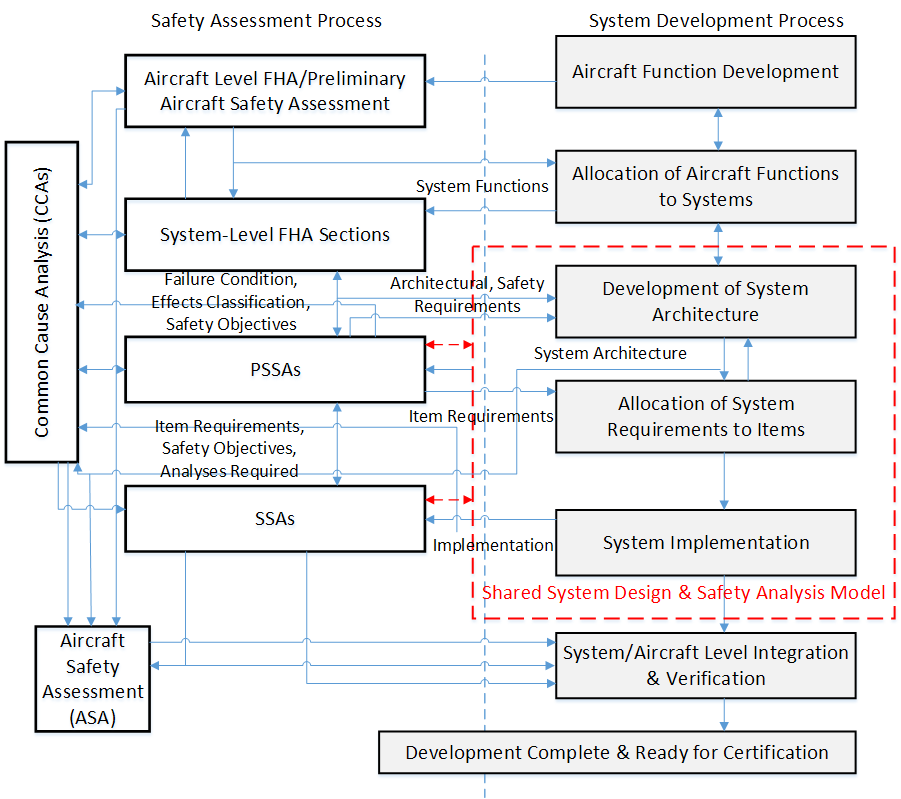
\includegraphics[trim=0 9 0 5,clip,width=0.85\textwidth]{images/Safety_Assessment_Process.png}
	%\vspace{0.4in}
	\caption{Using the Shared System/Safety Model in the ARP4754A Safety Assessment Process}
	\label{fig:proposed_safety_process}
\end{figure}

Figure~\ref{fig:proposed_safety_process} presents our proposed use of this shared system design and safety analysis model in the context of the ARP4754A Safety Assessment Process Model (derived from Figure 7 of ARP4754A). The shared model is one of the system development artifacts from the ``Development of System Architecture'' and ``Allocation of System Requirements to Item'' activities in the System Development Process, which interacts with the PSSAs and SSAs activities in the Safety Assessment Process. The shared model can serve as an interface to capture the information from the system design and implementation that is relevant for the safety analysis.

\begin{figure}[t!]
	\vspace{-0.19in}
	\centering
	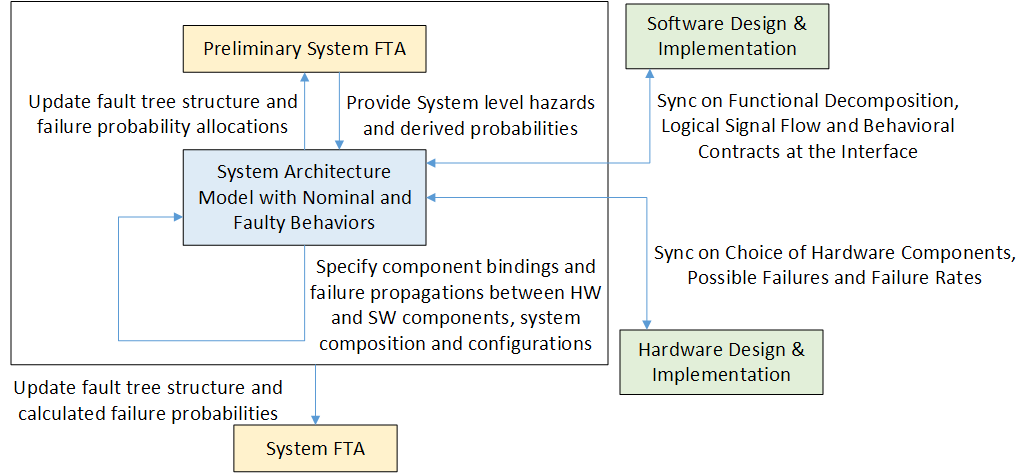
\includegraphics[width=0.9\textwidth]{images/FTA_MBD_Workflow.png}
	%\vspace{-0.19in}
	\caption{Example Interactions between the Shared System/Safety Model and the FTAs}
	\label{fig:interaction_with_FTA}
\end{figure}

Figure~\ref{fig:interaction_with_FTA} shows how the preliminary FTAs and final system FTAs (artifacts from the PSSA and SSA activities in the Safety Assessment Process) can guide and be updated from the shared model.
%\darren{Maybe we need a couple of sentences to explain what's happening in the figure.}
The shared model is expected to be created and maintained in sync with the software and hardware design and implementation, and guided by the hazard and probability information from the preliminary system FTA. The analysis results from checking the system level properties on the shared model are then used to update the preliminary system FTA. This process continues iteratively until the system safety property is satisfied with the desired fault tolerance and failure probability achieved. The effort needed to update the final system FTA from the preliminary system FTA would be greatly reduced.




\subsection{Modeling Language for System Design}
\label{subsec:aadl-agree}
Figure~\ref{fig:proposed_safety_process} presents our proposed use of a single unified model to support both system design and safety analysis. It describes both system design and safety-relevant information 
that are kept distinguishable and yet are able to interact with each other. The shared model is a living model that captures the current state of the system design as it moves through the development lifecycle, allowing all participants of the \gls{arp}4754A process to be able to communicate and review the system design. Safety related information can be generated directly through automated analysis on the model. This provides the capability to more accurately analyze complex systems. The generated safety information includes counterexamples which show causal failure scenarios and minimal sets of fault combinations that cause the failure condition to occur.

\begin{figure}[t!]
	
	\centering
	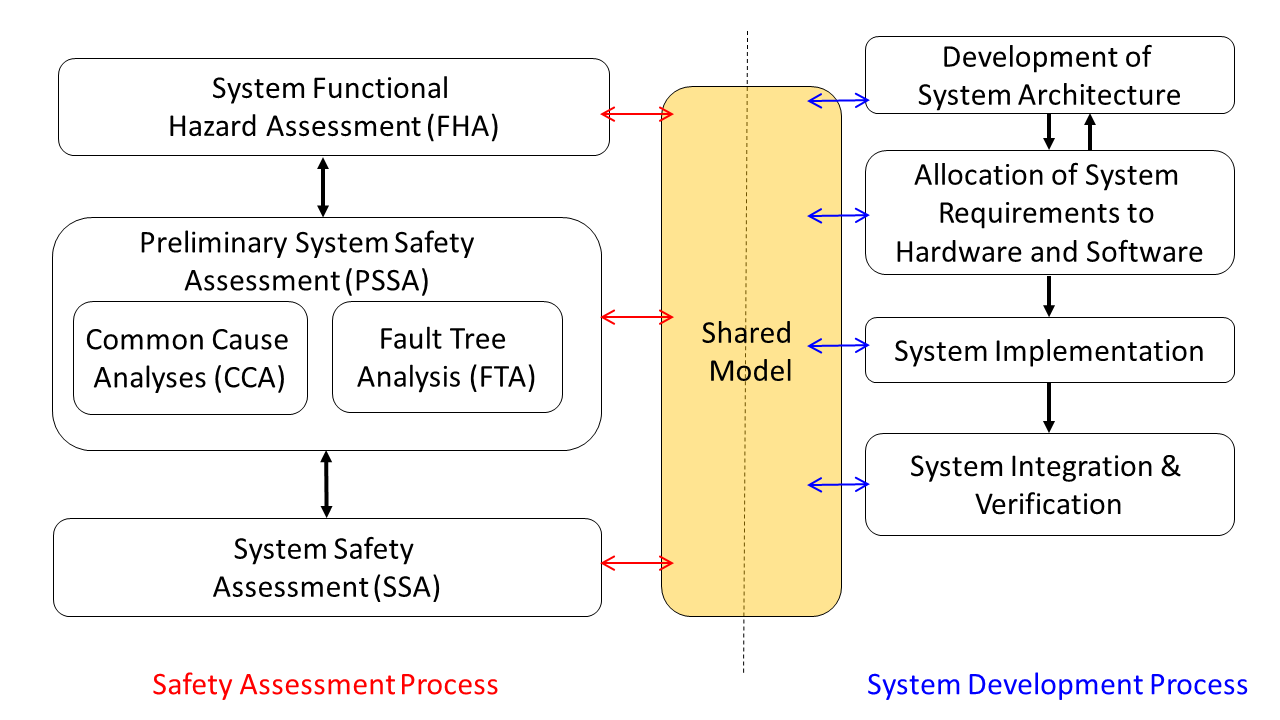
\includegraphics[trim=0 5 0 5,clip,width=0.85\textwidth]{images/process3.png}
	
	\caption{Use of the Shared System/Safety Model in the ARP4754A Safety Assessment Process}
	\label{fig:proposed_safety_process}
\end{figure}

We are using the Architectural Analysis and Design Language (AADL)~\cite{FeilerModelBasedEngineering2012} to construct system architecture models.  \gls{aadl} is an SAE International standard that defines a language and provides a unifying framework for describing the system architecture for ``performance-critical, embedded, real-time systems''~\cite{AADL_Standard}. From its conception, \gls{aadl} has been applied to the design and construction of avionics systems.  
Rather than being merely descriptive, \gls{aadl} models can be made specific enough to support system-level code generation.  Thus, results from analyses conducted, including the new safety analysis proposed here, correspond to the system that will be built from the model.  

An \gls{aadl} model describes a system in terms of a hierarchy of components and their interconnections, where each component can either represent a logical entity (e.g., application software functions, data) or a physical entity (e.g., buses, processors, memory). An \gls{aadl} model can be extended with language annexes to provide a richer set of modeling elements for various system design and analysis needs (e.g., performance-related characteristics, configuration settings, dynamic behaviors). The language definition is sufficiently rigorous to support formal analysis tools that allow for early phase error/fault detection.

The \gls{agree}~\cite{NFM2012:CoGaMiWhLaLu} is a tool for formal analysis of behaviors in \gls{aadl} models.  \gls{agree} is implemented as an \gls{aadl} annex and annotates \gls{aadl} components with formal behavioral contracts. Each component's contracts can include assumptions and guarantees about the component's inputs and outputs respectively, as well as predicates describing how the state of the component evolves over time. \gls{agree} translates an \gls{aadl} model and the behavioral contracts into Lustre~\cite{Halbwachs91:IEEE} and then queries the JKind
model checker~\cite{2017arXiv171201222G} to conduct the back-end analysis. The analysis %is
can be performed compositionally following the architecture hierarchy such that analysis at a higher level is based on the components at the next lower level.  When compared to monolithic analysis (i.e., analysis of the flattened model composed of all components), the compositional approach allows the analysis to scale to much larger systems~\cite{NFM2012:CoGaMiWhLaLu}. 

%In the avionics context, the software functions/applications, the hardware equipment, and the system that is composed of their integration can all be represented as components connected to/composed of/bind to other components in a hierarchical AADL model. AGREE contracts can be used to capture the functional requirements at each level of the hierarchy. Once the model has been reviewed and the requirements captured have been validated, the back-end analysis can be conducted to verify if each level of the model implements its higher level requirements correctly.

%AADL with the AGREE extension serves as a good candidate as the modeling language for describing the system design aspects of a shared system design and safety analysis model. 
%In our prior work~\cite{Stewart17:IMBSA}, we added an initial failure effect modeling capability to the AADL/AGREE language and tool set.  We are continuing this work so that our tools and methodology can be used to satisfy system safety objectives of ARP4754A and ARP4761.  

\begin{comment}
In particular, our goals are to:

\begin{itemize}
	\item Provide a comprehensive, qualitative description of the causal relationship between basic failure events and system level safety requirements.
	\item Provide an accurate, quantitative description of the contribution relationship between failure rates of the fault tree basic events and numerical probability requirements at the system level.
\end{itemize}
\end{comment}
%The remainder of the paper describes our approach towards both of the goals.





\subsection{Model-Based Safety Assessment Process Supported by Formal Methods}
\label{subsec:process}
We propose a model-based safety assessment process backed by formal methods to help safety engineers with early detection of the design issues.  This process uses a single unified model to support both system design and safety analysis. It is based on the following steps:

\begin{enumerate}
	\item System engineers capture the critical information in a shared AADL/AGREE model:  high-level hardware and software architecture, nominal behavior at the component level, and safety requirements at the system level.% (e.g., inhibit throttle movement during critical takeoff phase).
	\item System engineers use the backend model checker to verify that the safety requirements are satisfied by the nominal design model. 
	\item Safety engineers use the Safety Annex to augment the nominal model with the component failure modes. % (e.g., processor failure, input signal corrupted).  
	In addition, safety engineers specify the fault hypothesis for the analysis which corresponds to how many simultaneous faults the system must be able to tolerate.
	\item Safety engineers use the backend model checker to analyze if the safety requirements and fault tolerance objectives are satisfied by the design in the presence of faults. % (e.g., if the system is resilient to a single failure). 
	If the design does not tolerate the specified number of faults (or probability threshold of fault occurrence), then the tool produces counterexamples leading to safety requirement violation in the presence of faults, %and also
	 as well as all minimal set of fault combinations that can cause the safety requirement to be violated.
	%produces fault trees showing smallest set of faults that may lead to the safety requirement being violated. 
	\item The safety engineers examine the results to assess the validity of the fault combinations and the fault tolerance level of the system design. If a design change is warranted, the model will be updated with the latest design change and the above process is repeated.
\end{enumerate}

There are other tools purpose-built for safety analysis, including AltaRica~\cite{PROSVIRNOVA2013127}, smartIFlow~\cite{info8010007} and xSAP~\cite{DBLP:conf/tacas/BittnerBCCGGMMZ16}. These tools and their accompanying notations are separate from the system development model. Other tools extend existing system models, such as HiP-HOPS~\cite{CHEN201391} and the AADL Error Model Annex, Version 2 (EMV2)~\cite{EMV2}. EMV2 uses enumeration of faults in each component and explicit propagation of faulty behavior to perform error analysis. The required propagation relationships must be manually added to the system model and can become complex and lead to mistakes in the analysis.

In contrast, the Safety Annex supports model checking and quantitative reasoning by attaching behavioral faults to components and then using the normal behavioral propagation and proof mechanisms built into the AGREE AADL annex.  This allows users to reason about the evolution of faults over time, and produce counterexamples demonstrating how component faults lead to failures.
Our approach adapts the work of Joshi et. al
~\cite{Joshi05:Dasc} to the AADL modeling language.  Stewart, et. al provide more information on the approach~\cite{Stewart17:IMBSA}, and the tool and relevant documentation can be found at: \small \url{https://github.com/loonwerks/AMASE/}. \normalsize

%\subsection{Comparison with EMV2}
\label{subsec:comparison_with_EMV2}

The AADL language has previously been extended to provide some fault modeling and analysis capabilities using its Error Model Annex, Version 2 (EMV2)~\cite{EMV2}.  EMV2 focuses on injection and propagation of discrete faults for generation of fault trees, rather than on analysis of system behavior in the presence of faults. In order for a component to have an impact on the rest of the system, all faults must be explicitly propagated through each component by applying fault types on each of the output ports. When using this type of fault analysis, the safety analyst must understand the system  behavior and component functions well enough to specify how a failure will propogate through the system, what the destination components reaction to said failure will be, and correctly implement these propagations. In EMV2, every possible component failure must be specified in this way. As a contrast, the Safety Annex provides two ways in which to specify these faults. The explicit propagation capability in the Safety Annex is meant to capture hardware faults and faults that occur due to colocated components. In every other instance, implicit propagation is used through the behavior model. In related work, comparisons with other related toolsets is explored in more depth. 














\iffalse

The AADL language has previously been extended to provide some fault modeling and analysis capabilities using its Error Model Annex, Version 2 (EMV2)~\cite{EMV2}.  EMV2 focuses on injection and propagation of discrete faults for generation of fault trees, rather than on analysis of system behavior in the presence of faults. 
To illustrate some of the key differences between our approach and the EMV2 approach, Figure~\ref{fig:comparison_with_EMV2} shows a simplified example based on an aircraft Wheel Brake System (WBS). The WBS model is described in greater detail in ~\cite{Stewart17:IMBSA} and in Section \ref{sec:case_study}. The code fragments in the figure extracted from EMV2, AGREE, and the Safety Annex do not represent the complete code.

\begin{figure}[t]
	\vspace{-0.19in}
	\centering
	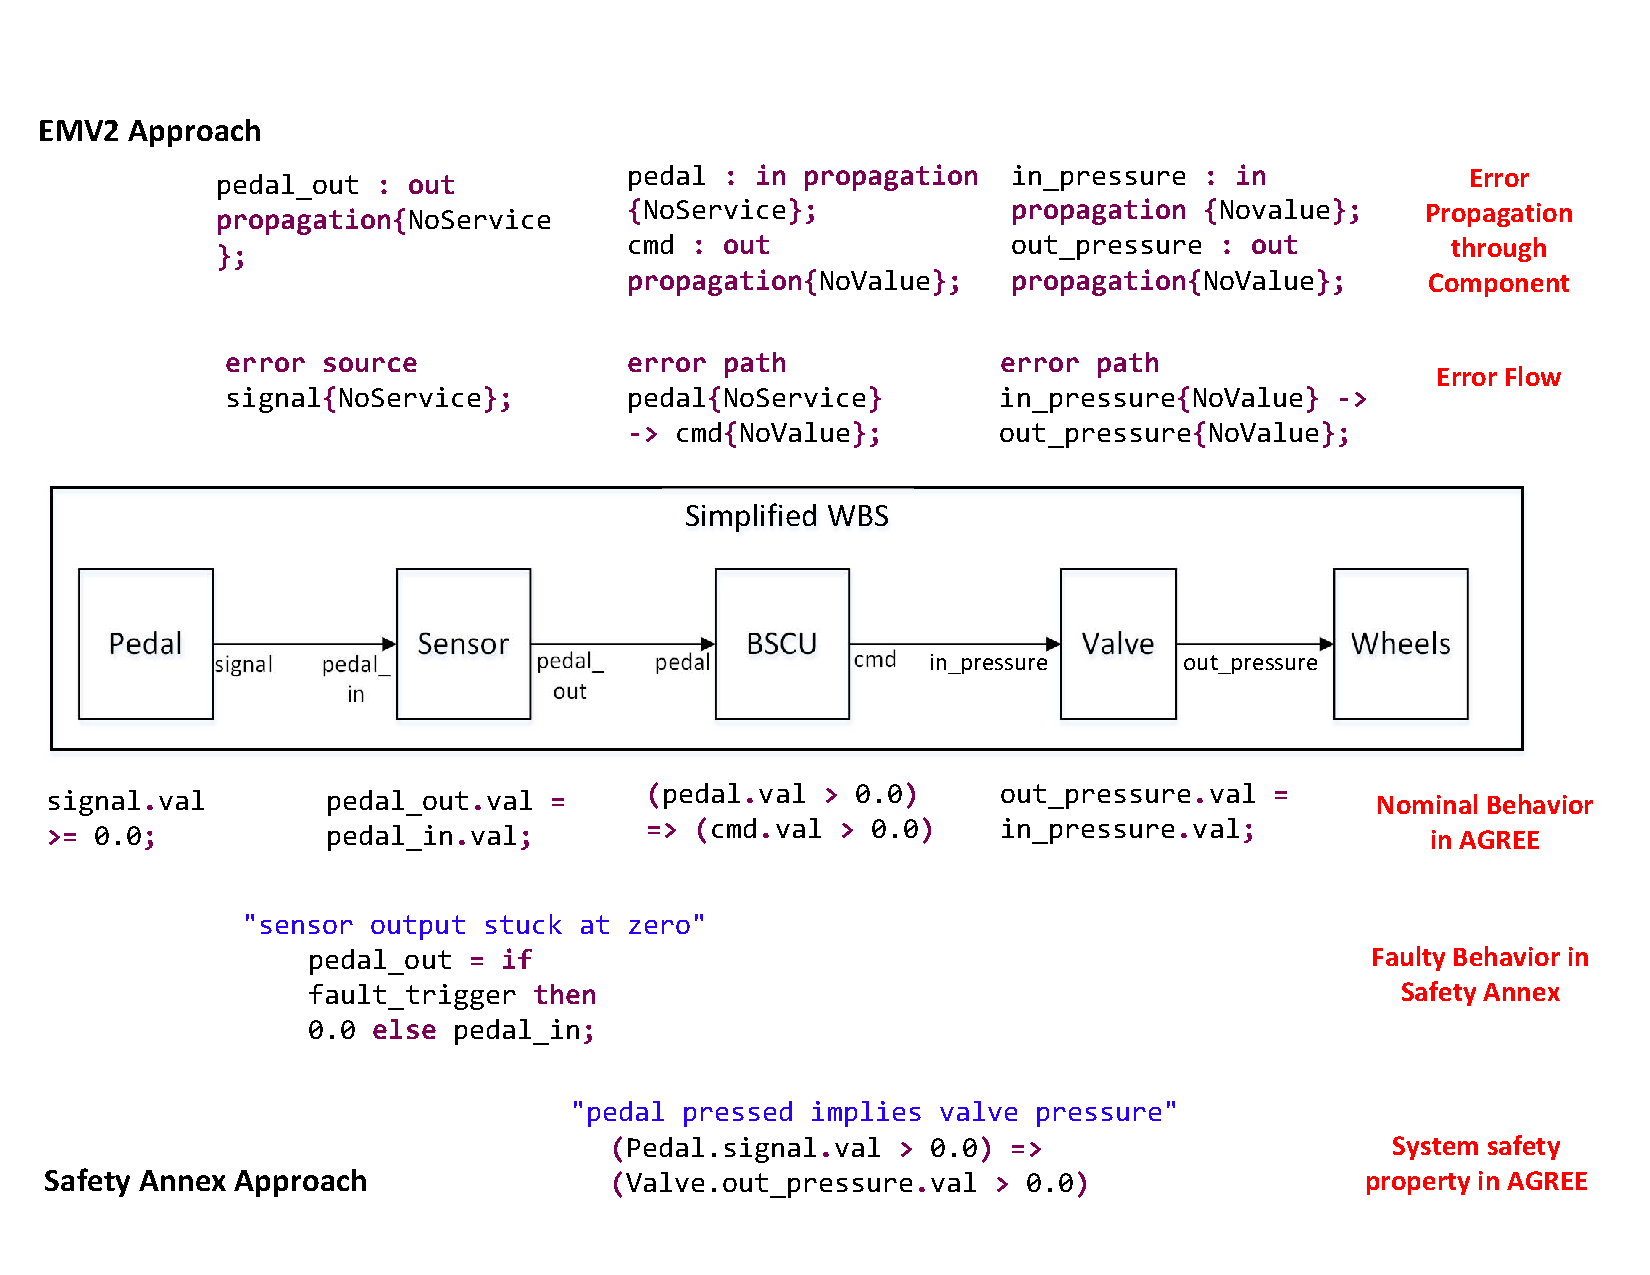
\includegraphics[trim=0 9 0 5,clip,width=\textwidth]{images/Comparison_with_EMV2.pdf}
	%\vspace{0.4in}
	\caption{Differences between Safety Annex and EMV2}
	\label{fig:comparison_with_EMV2}
\end{figure} 

In our simplified WBS system, the physical signal from the Pedal component in detected by the Sensor, and the pedal position value is passed to the Braking System Control Unit (BSCU) components.  The BSCU generates a pressure command to the Valve component which applies hydraulic brake pressure to the Wheels. In this example, we use the general term ``fault'' to denote all component errors, hardware failures, and system faults captured by both approaches.

In the EMV2 approach (top half of Figure~\ref{fig:comparison_with_EMV2}), all faults must be explicitly propagated through each component (by applying fault types on each of the output ports) in order for a component to have an impact on the rest of the system. In the example, the ``NoService'' fault is explicitly allowed by the EMV2 declarations to propagate through all of the components.  These fault types are essentially tokens that do not capture any analyzable behavior.  At the system level, analysis tools supporting the EMV2 annex can aggregate the fault flow and propagation information from different components to compose an overall fault flow diagram or fault tree.

In the Safety Annex approach (bottom half of Figure~\ref{fig:comparison_with_EMV2}), faults are captured as faulty behaviors that augment the system behavioral model in AGREE contracts.  When a fault is triggered, the output behavior of the Sensor component is modified, in this case resulting a ``stuck at zero'' error. The behavior of the BSCU receives a zero input and proceeds as if the pedal has not been pressed. This will cause the top level system contract to fail: {\em pedal pressed implies brake pressure output is positive}. No explicit fault propagation is necessary since the faulty behavior itself propagates through the system just as in the nominal system model. The effects of any triggered fault are manifested through analysis of the AGREE contracts. 


 \fi





%\subsection{Comparison with Proposed MBSA Appendix to ARP4761A}
\label{sec:mbsa_appendix_review}

ARP4754A, the Guidelines for Development of Civil Aircraft and Systems~\cite{SAE:ARP4754A}, provides guidance on applying development assurance at each hierarchical level throughout the development life cycle of highly-integrated/complex aircraft systems. ARP4761, the Guidelines and Methods for Conducting Safety Assessment Process on Civil Airborne Systems and Equipment~\cite{SAE:ARP4761},  identifies a systematic means to show compliance. A Model Based Safety Analysis (MBSA) appendix has been drafted to the upcoming revision of ARP4761 to provide concepts and processes with Model Based Safety Analysis.

We have reviewed the draft appendix and found that our approach is consistent with the MBSA appendix in the following ways:

\begin{itemize}
	\item The common goal is to use MBSA for an equivalent analysis to the traditional safety analysis methods (e.g., Fault Trees) to support safety assessment processes.
	\item Both use an analytical model of the system to capture failure propagation. In the model, system architecture, nominal and faulty functional behaviors are captured. The model evolves as the system design evolves.
	\item Both use software application/tools to perform analysis on the model and generate outputs (e.g., failure sequences, minimal cut sets that result in the failure condition under analysis). The MBSA appendix also mentioned that model checking can be used to perform an exhaustive exploration of the state space of the model.
	\item Outputs generated from the analysis are to be compared to qualitative and/or quantitative objectives and requirements as part of the safety assessment process. Furthermore, the outputs drive evolution of system design. 
\end{itemize}

Our approach goes beyond what is envisioned in the MBSA appendix in the following ways:

\begin{itemize}
	\item The MBSA Appendix is not advocating a single unified model used by both system development and safety assessment activities. The model is safety specific and driven by the types of safety assessment to be conducted. However, the initial safety model may be derived from the system design model, and may be closer to the design at the lower levels of the design process.
	\item In the MBSA Appendix, the failure propagation modeling focuses on the inside internal flows in the components, which is similar to the bottom-up method in Failure Modes and Effects Analysis. Different components are connected by inputs and outputs, and no behavioral constraints are specified on data entering and exiting components. This leaves inter-component propagation to be explored by the analysis.
\end{itemize}

In summary, our approach provides a new way to do safety analysis. It uses an unified model that is shared by system development and safety assessment. The model captures architecture and behavioral information for propagation within components and between components. It is a property driven approach that is consistent between system verification and safety analysis.










































\section{Fault Modeling with the Safety Annex}
\label{sec:fault_modeling}

To demonstrate the fault modeling capabilities of the Safety Annex we will use the Wheel Brake System (WBS) described in AIR6110~\cite{AIR6110}.  This system is a well-known example that has been used as a case study for safety analysis, formal verification, and contract based design~\cite{DBLP:conf/cav/BozzanoCPJKPRT15, 10.1007/978-3-319-11936-6-7, CAV2015:BoCiGrMa, Joshi05:SafeComp}. The preliminary work for the safety annex was based on a simple model of the WBS~\cite{Stewart17:IMBSA}. To demonstrate a more complex fault modeling process, we constructed a functionally and structurally equivalent AADL version of the more complex WBS NuSMV/xSAP models~\cite{DBLP:conf/cav/BozzanoCPJKPRT15}, as illustrated in Figure \ref{fig:inadvertent_braking}.     

\begin{figure*}[t]
	\centering
	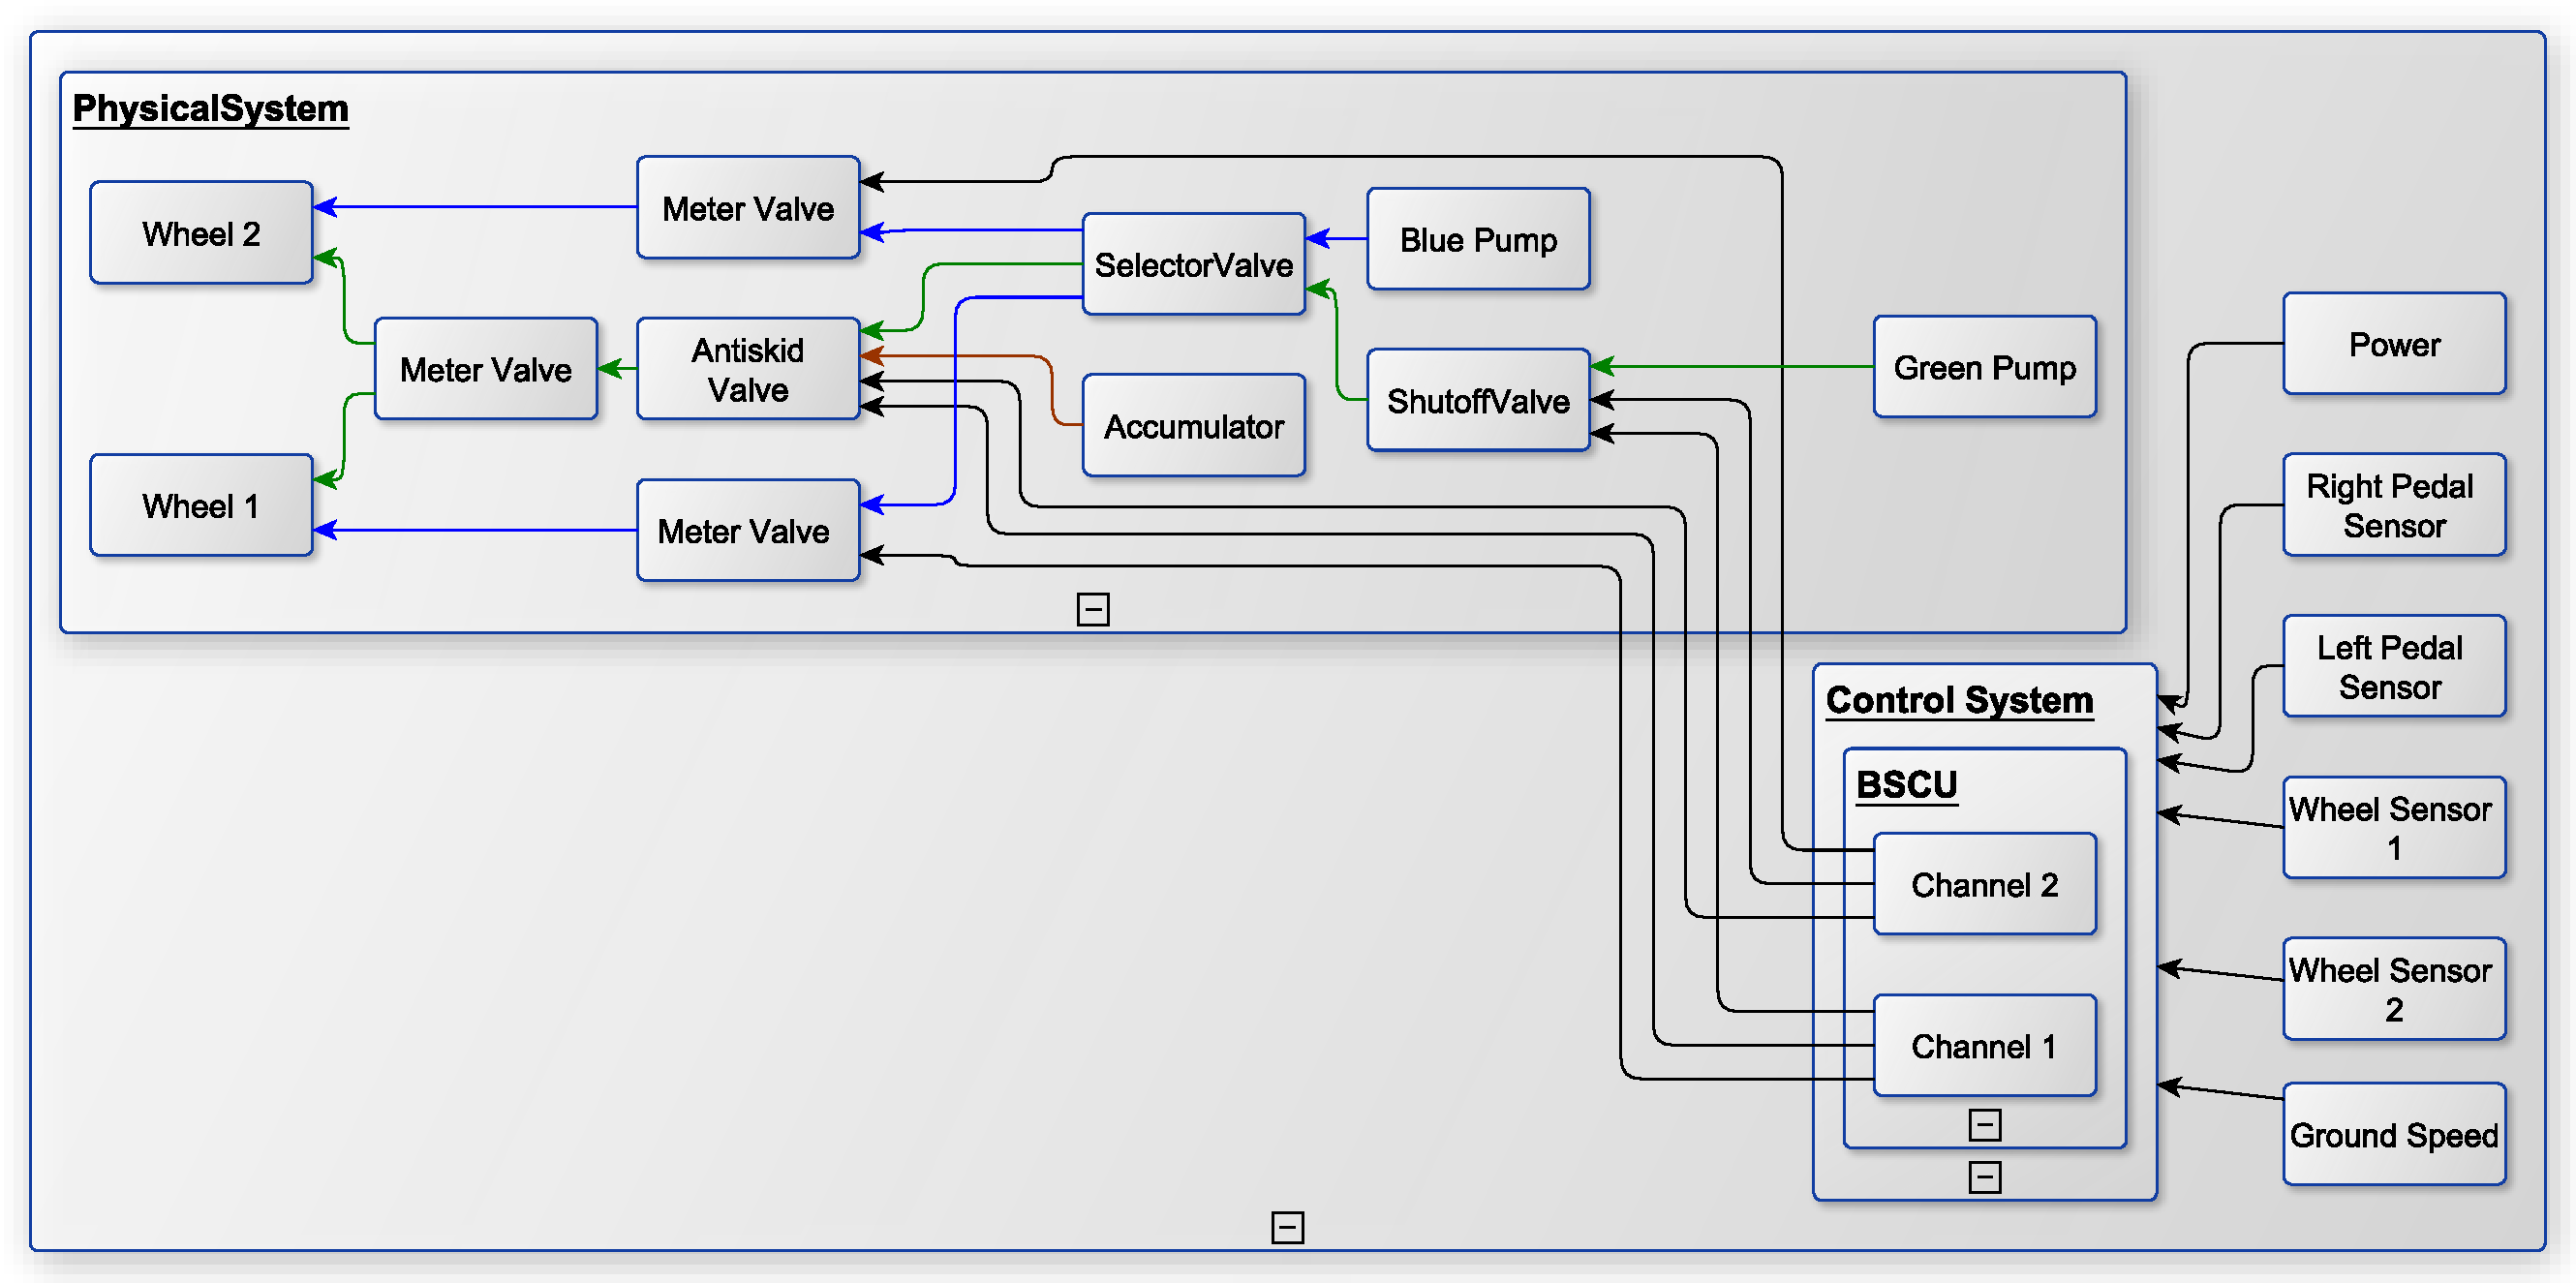
\includegraphics[trim=0 9 0 5,clip,width=.7\dimexpr\textwidth-2cm\relax]{images/wbs_arch4_diagram.pdf}
	\caption{Wheel Brake System}
	\label{fig:wbs}
\end{figure*} 


The WBS is composed of two main parts: the Line Replaceable Unit control system and the electro-mechanical physical system.
The control system electronically controls the physical system and contains a redundant
channel of the Braking System Control Unit (BSCU) in case a detectable fault occurs in the active channel.
 It also commands antiskid braking. % in case of skidding on the ground. 
 The physical system consists of the hydraulic circuits running from hydraulic pumps to wheel brakes as well as valves that control the hydraulic fluid flow. This system provides braking force to each of the eight wheels of the aircraft. The wheels are all mechanically braked in pairs (one pair per landing gear). For simplicity, Figure~\ref{fig:wbs} displays only two of the eight wheels. 

There are three operating modes in the WBS model:

\begin{itemize}
	\renewcommand{\labelitemi}{\textbullet}
	\item In \textit{normal} mode, the system is composed of a \textit{green} hydraulic pump and one meter valve per each of the eight wheels. Each of the meter valves are controlled through electronic commands coming from the active channel of the BSCU. These signals provide braking and antiskid commands for each wheel. The braking command is determined through a sensor on the pedal and the antiskid command is determined by the \textit{Wheel Sensors}. 
	\item In \textit{alternate} mode, the system is composed of a \textit{blue} hydraulic pump, four meter valves, and four antiskid shutoff valves, one for each landing gear. The meter valves are mechanically commanded through the pilot pedal corresponding to each landing gear. There are two ways the system can change into alternate mode. The selector can choose the blue circuit when the BSCU sends a system invalid signal, or the system can switch to the blue circuit when the selector detects lack of pressure in the green circuit.
	%There are two ways the system can change into alternate mode. Either the selector detects lack of pressure in the green circuit and switches to the blue circuit or the BSCU sends a validity signal to the selector in which case the selector chooses the blue line.
	\item In \textit{emergency} mode, the system mode is entered if the \textit{blue} hydraulic pump fails. The accumulator pump has a reserve of pressurized hydraulic fluid and will supply this to the blue circuit in emergency mode. 
\end{itemize}

The WBS architecture model in AADL contains 30 different kinds of components, 169 component instances, and a model depth of 5 hierarchical levels. 


%If the BSCU channel becomes invalid, the shutoff valve closes and we move into alternate mode. Once this system switches into alternate mode, it does not return to normal operation mode.

%There are three operating modes in the WBS model. In \textit{normal} mode, the system uses the \textit{green} hydraulic circuit. The normal system is composed of the green hydraulic pump and one meter valve per each of the eight wheels. Each of the meter valves are controlled through electronic commands coming from the active channel of the BSCU. These signals provide braking and antiskid commands for each wheel. The braking command is determined through a sensor on the pilot pedal position and is labeled as \textit{Left/Right Pedal Sensor} in Figure~\ref{fig:wbs} and the antiskid command is determined by the \textit{Wheel Sensors}. 

%In \textit{alternate} mode, the system uses the \textit{blue} hydraulic circuit. The alternate system is composed of the blue hydraulic pump, four meter valves, and four antiskid shutoff valves: one for each landing gear. The meter valves are mechanically commanded through the pilot pedal corresponding to each landing gear. If the system detects lack of pressure in the green circuit, the BSCU channel commands the selector valve to switch to the blue circuit. 
%If the BSCU channel becomes invalid, the shutoff valve closes and we move into alternate mode. Once this system switches into alternate mode, it does not return to normal operation mode.

%The last mode of operation of the WBS is the \textit{emergency} mode. This mode is entered if the blue hydraulic pump fails. The accumulator pump has a reserve of pressurized hydraulic fluid and will supply this to the blue circuit in emergency mode.

%The model contains 30 different kinds of components, 169 component instances, a model depth of 5 hierarchical levels.  The model includes one top-level assumption and  11 top-level system properties, with 113 guarantees allocated to subsystems.  There are a total of 33 different fault types and 141 fault instances within the model.  The large number of fault instances is due to the redundancy in the system design and its replication to control 8 wheels.

The behavioral model is encoded using the AGREE annex and the behavior is based on descriptions found in AIR6110. The top level system properties are given by the requirements and safety objectives in AIR6110. All of the subcomponent contracts support these system safety objectives through the use of assumptions on component input and guarantees on the output. The WBS behavioral model in AGREE annex includes one top-level assumption and  11 top-level system properties, with 113 guarantees allocated to subsystems.  

An example system safety property is to ensure that there is no inadvertent braking of any of the wheels. This is based on a failure condition described in AIR6110 is \textit{Inadvertent wheel braking on one wheel during takeoff shall be less than %1E-9 
$1.0\times 10^{-9}$ per takeoff}. 
Inadvertent braking means that braking force is applied at the wheel but the pilot has not pressed the brake pedal.  In addition, the inadvertent braking requires that power and hydraulic pressure are both present, the plane is not stopped, and the wheel is rolling (not skidding). The property is stated in AGREE such that inadvertent braking does \textit{not} occur, as shown in Figure \ref{fig:inadvertent_braking}. 

\begin{figure}[h!]
	%\vspace{-0.2in}
	\begin{center}
	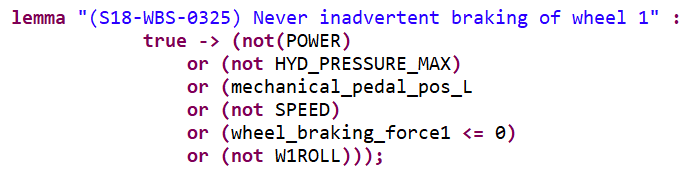
\includegraphics[width=.9\columnwidth]{images/inadvertent_braking.png}
	\end{center}
	%\vspace{-0.3in}
	\caption{AGREE Contract for Top Level Property: Inadvertent Braking}
	\label{fig:inadvertent_braking}
	\vspace{-0.2in}
\end{figure}


\subsection{Component Fault Modeling}

The usage of the terms error, failure, and fault are defined in ARP4754A and are described here for clarity
%ease of understanding
~\cite{SAE:ARP4754A}. An \textit{error} is a mistake made in implementation, design, or requirements. A \textit{fault} is the manifestation of an error and a \textit{failure} is an event that occurs when the delivered service of a system deviates from correct behavior. If a fault is activated under the right circumstances, that fault can lead to a failure. The terminology used in EMV2 differs slightly for an error: an error is a corrupted state caused by a fault. The error propagates through a system and can  manifest as a failure. In this paper we use the ARP4754A terminology with the added definition of \textit{error propagation} as used in EMV2. An error is a mistake made in design or code and an error propagation is the propagation of the corrupted state caused by an active fault. 

The Safety Annex is used to add possible faulty behaviors to a component model. Within the AADL component instance model, an annex is added which contain the fault definitions for the given component. The flexibility of the fault definitions allows the user to define numerous types of fault \textit{nodes} by utilizing the AGREE node syntax. A library of common fault nodes has been written and is available in the project GitHub repository~\cite{SAGithub}. Examples of such faults include valves being stuck open or closed, output of a software component being nondeterministic, or power being cut off.  When the fault analysis requires fault definitions that are more complex, these nodes can easily be created and used in the model. 
%\janet{Since AADL models is an abstract representation of the system, expected and faulty behaviors from the operators could also be modeled in AGREE and Safety Annex.}

When a fault is activated by its specified triggering conditions, it modifies the output of the component. This faulty behavior may lead to the violation of the contracts of other components in the system, including assumptions of downstream components. The impact of a fault is computed by the AGREE model checker when the safety analysis is run on the fault model. 

The majority of faults that are connected to outputs of components are known as \textit{symmetric}. That is, whatever components receive this faulty output will receive the same faulty output value. Thus, this output is seen symmetrically. An alternative fault type is \textit{asymmetric}. This pertains to a component with a 1-n output: one output which is sent to many receiving components. This fault can present itself differently to the receiving components. For instance, in a boolean setting, one component might see a true value and the rest may see false. This type of fault is modeled using the keyword \textit{asymmetric}. For more information on fault definitions and modeling possibilities, we refer readers to the Safety Annex Users Guide\cite{SAGithub}. %\danielle{This might be all we need for mentioning asym faults...}

As an illustration of fault modeling using the Safety Annex, we look at one of the components relevant to the inadvertent braking property: the brake pedal. When the mechanical pedal is pressed, a sensor reads this information and passes an electronic signal to the BSCU that then commands hydraulic pressure to the wheels. 

\begin{comment}
%Figure~\ref{fig:sensor} 
Figure~\ref{fig:sensor} shows the AADL pedal sensor component with a contract for its nominal behavior. The sensor has only one input, the mechanical pedal position, and one output, the electrical pedal position. 
A property that governs the behavior of the component is that the mechanical position should always equal the electronic position. (The expression \textit{true $\rightarrow$ property} in AGREE is true in the initial state and then afterwards it is only true if property holds.)

\begin{figure}[h!]
	%\hspace*{-2cm}
	%\vspace{-0.55in} 
	\begin{center}
		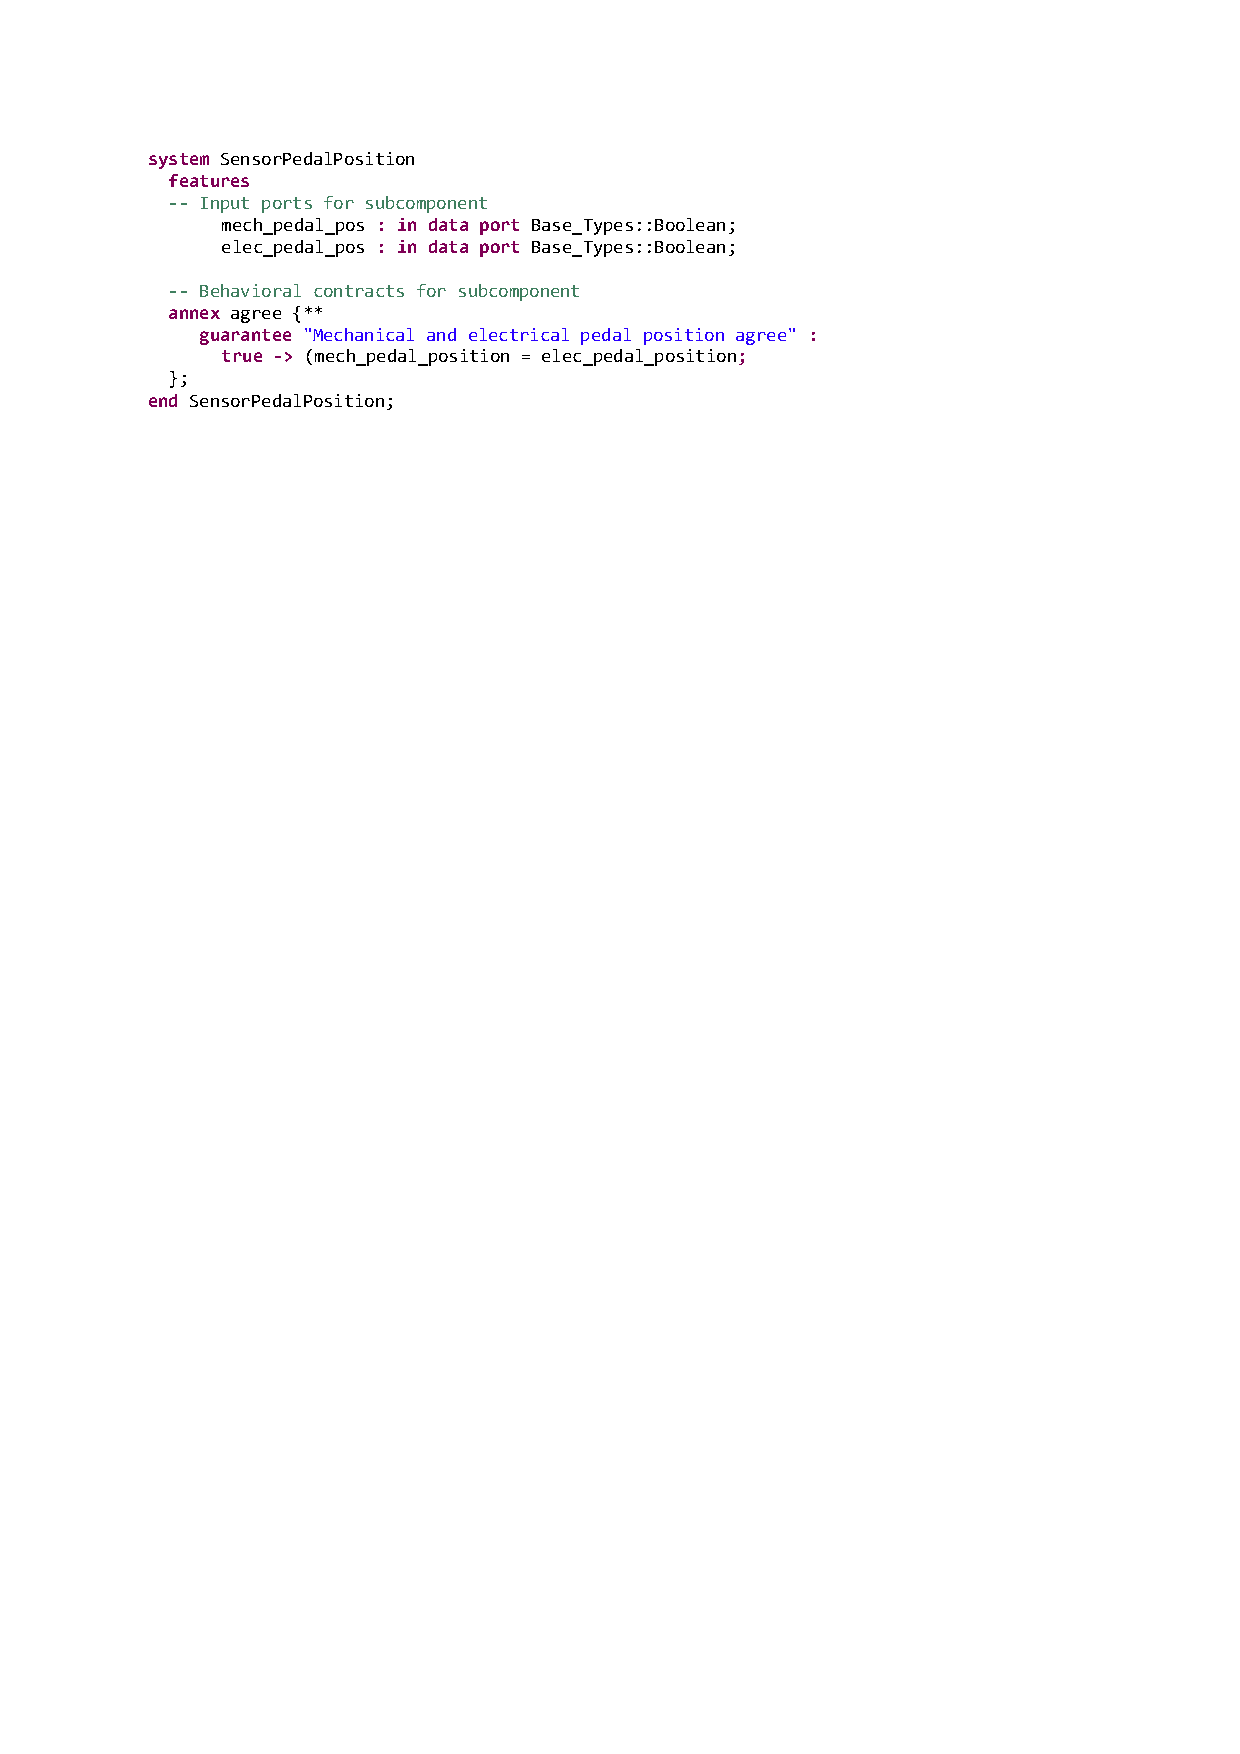
\includegraphics[trim=0 640 -10 70,clip,width=.8\dimexpr\textwidth-2cm\relax]{images/system_sensor.pdf}
		%\vspace{-0.3in}
		\caption{An AADL System Type: The Pedal Sensor}
		\label{fig:sensor}
	\end{center}
	\vspace{-0.2in}
\end{figure}
\end{comment}

One possible failure for this sensor is inversion of its output value. This fault can be triggered with probability $5.0\times 10^{-6}$ as described in AIR6110 (in reality, the component failure probability is 
collected from hardware specification sheets).  
The Safety Annex definition for this fault is shown in Figure~\ref{fig:sensorFault}. Fault behavior is defined through the use of a fault node called \textit{inverted\_fail}.  When the fault is triggered, the nominal output of the component (\textit{elec\_pedal\_position}) is replaced with its failure value (\textit{val\_out}). 

\begin{figure}[h!]
	%\hspace*{-2cm}
	%\vspace{-0.5in} 
	\begin{center}
		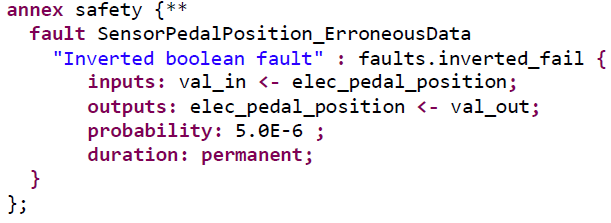
\includegraphics[width=.9\columnwidth]{images/safetyannex_sensorfault.png}
		%\vspace{-0.2in}
		\caption{The Safety Annex for the Pedal Sensor}
		\label{fig:sensorFault}
	\end{center}
	\vspace{-0.1in}
\end{figure}

The WBS fault model expressed in the Safety Annex contains a total of 33 different fault types and 141 fault instances. The large number of fault instances is due to the redundancy in the system design and its replication to control 8 wheels.

\subsection{Implicit Error Propagation}
In the Safety Annex approach, faults are captured as faulty behaviors that augment the system behavioral model in AGREE contracts. Unlike AADL EMV2, no explicit %fault
error propagation is necessary since the faulty behavior itself propagates through the nominal behavior contracts of the non-failed system components. The effects of any triggered fault are manifested through analysis of the AGREE contracts.  

%On the contrary, in the AADL Error Model Annex, Version 2 (EMV2)~\cite{EMV2} approach, all errors must be explicitly propagated through each component (by applying fault types on each of the output ports) in order for a component to have an impact on the rest of the system. To illustrate the key differences between implicit %failure
%error propagation provided in the Safety Annex and the explicit %failure 
%error propagation provided in EMV2, we use a simplified behavioral flow from the WBS example using code fragments from EMV2, AGREE, and the Safety Annex. 

\begin{figure*}[t]
	%\hspace*{-2cm}
	%\vspace{-0.19in}
	\centering
	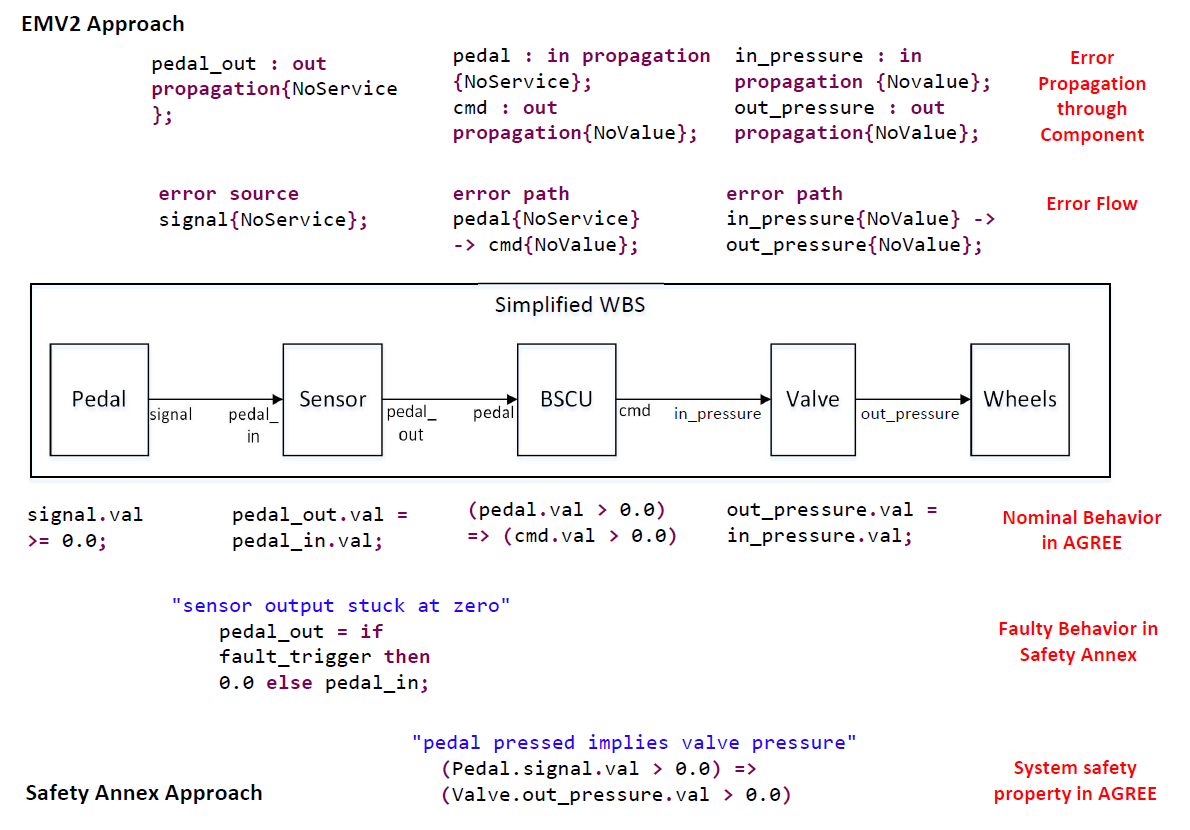
\includegraphics[width=0.7\textwidth]{images/Comparison_with_EMV2.png}
	%\vspace{-0.3in}
	\caption{Differences between Safety Annex and EMV2}
	\label{fig:comparison_with_EMV2}
	%\vspace{-0.2in}
\end{figure*} 

To illustrate key differences between implicit error propagation in the Safety Annex and explicit propagation in  EMV2, we use a simple example derived from the WBS, shown in Figure~\ref{fig:comparison_with_EMV2}. 
In this simplified WBS system, the physical signal from the Pedal component is detected by the Sensor and the pedal position value is passed to the Braking System Control Unit (BSCU) components.  The BSCU generates a pressure command to the Valve component which applies hydraulic brake pressure to the Wheels. 

In the EMV2 approach (top half of Figure~\ref{fig:comparison_with_EMV2}), the ``NoService'' fault is explicitly propagated through all of the components. These fault types are essentially tokens that do not capture any analyzable behavior. At the system level, analysis tools supporting the EMV2 annex can aggregate the propagation information from different components to compose an overall fault flow diagram or fault tree. 

The Safety Annex is used to add failure behaviors to the Sensor and Valve components and to specify the fault hypothesis (in this case, a single fault). 
When a fault condition is triggered in the analysis, the output behavior of that component is produced by its failure contract instead of its nominal contract.  For our simplified example, if the Sensor component fault condition is triggered, the result is a ``stuck at zero'' error. The contract of the BSCU receives a zero input and proceeds as if the pedal has not been pressed. This will cause the top level system contract to fail.

\begin{comment}
%\subsection{Comparison to the AADL Error Annex}

The AADL language has previously been extended to provide some fault modeling and analysis capabilities using its Error Model Annex, Version 2 (EMV2)~\cite{EMV2}.  EMV2 focuses on injection and propagation of discrete faults for generation of fault trees, rather than on analysis of system behavior in the presence of faults. 
To illustrate some of the key differences between our approach and the EMV2 approach, Figure~\ref{fig:comparison_with_EMV2} shows a simplified  behavioral flow with code fragments from EMV2, AGREE, and the Safety Annex. 

\begin{figure}[t]
	\vspace{-0.45in}
	\centering
	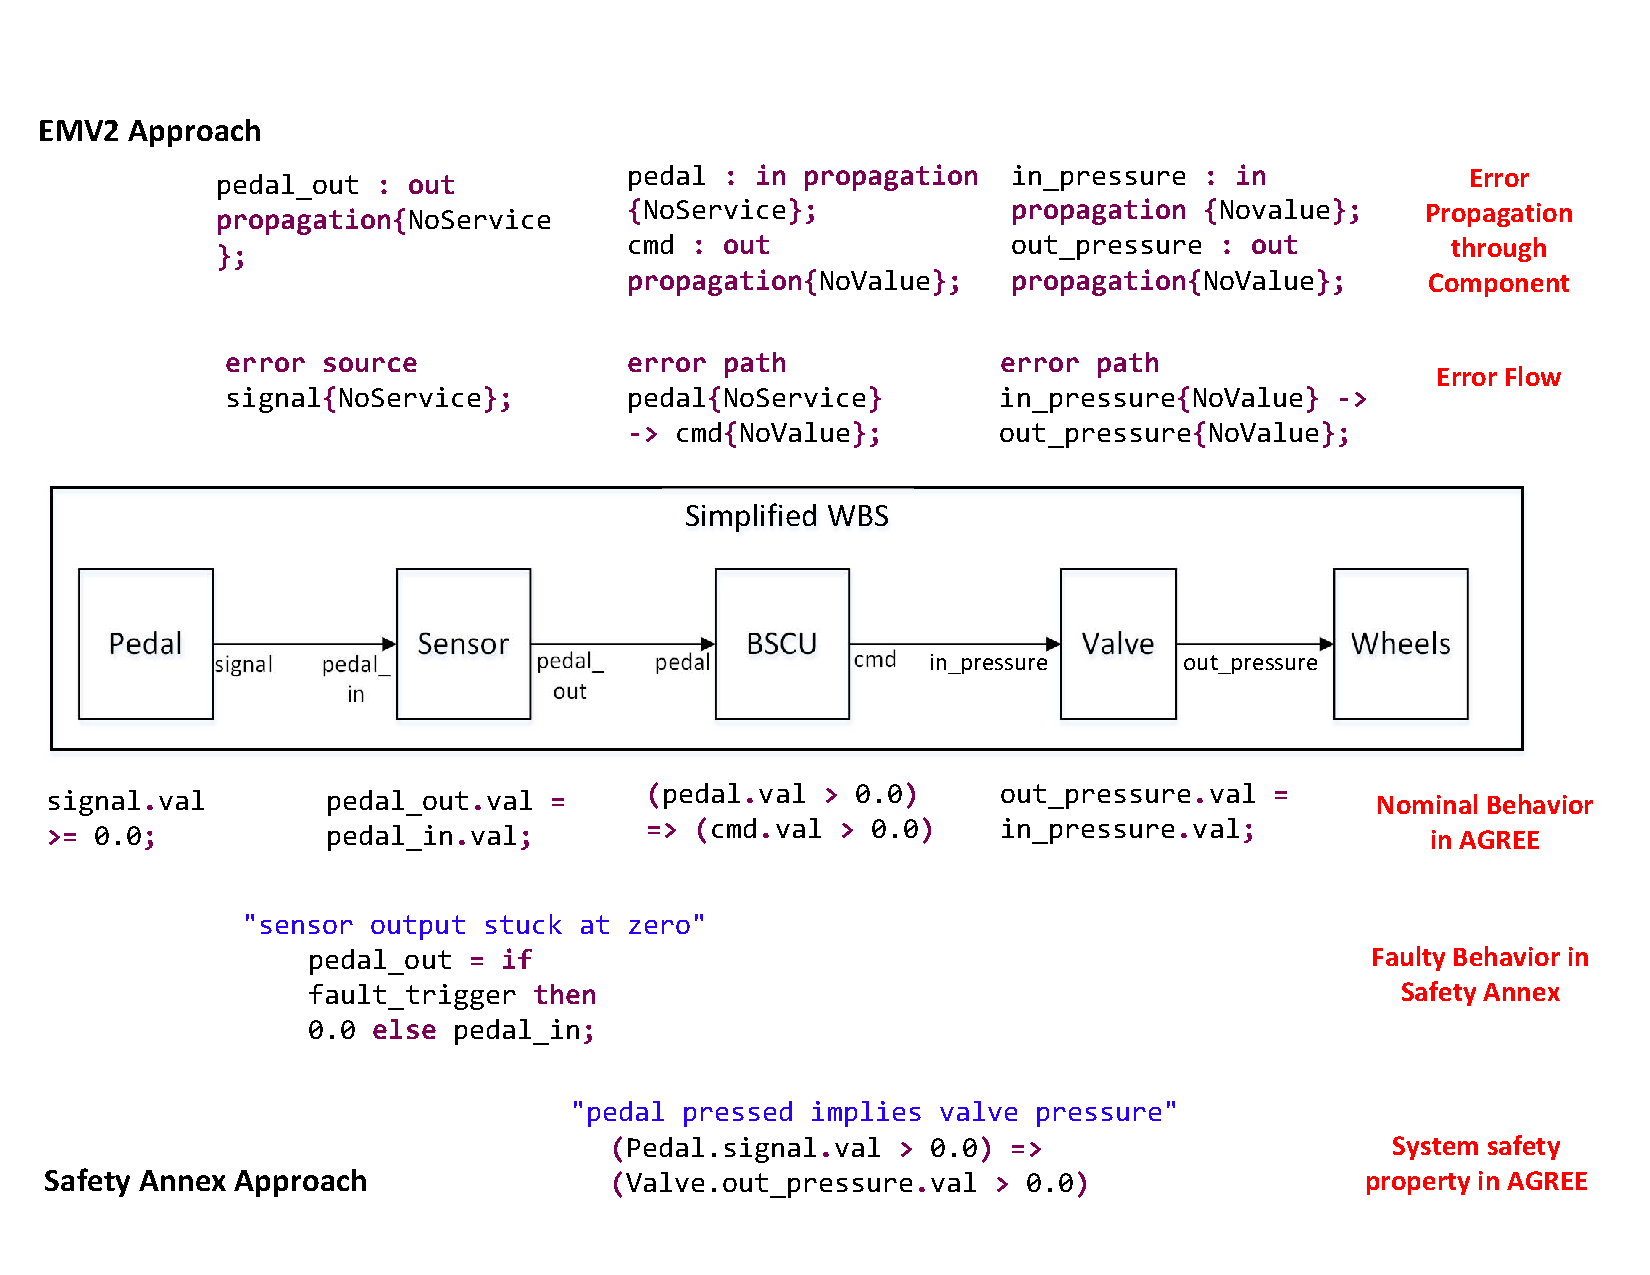
\includegraphics[trim=0 9 0 5,clip,width=.8\dimexpr\textwidth-2cm\relax]{images/Comparison_with_EMV2.pdf}
	%\vspace{0.4in}
	\caption{Differences between Safety Annex and EMV2}
	\label{fig:comparison_with_EMV2}
\end{figure} 

In this simplified WBS system, the physical signal from the Pedal component is detected by the Sensor, and the pedal position value is passed to the Braking System Control Unit (BSCU) components.  The BSCU generates a pressure command to the Valve component which applies hydraulic brake pressure to the Wheels. 

In the EMV2 approach (top half of Figure~\ref{fig:comparison_with_EMV2}), all errors must be explicitly propagated through each component (by applying fault types on each of the output ports) in order for a component to have an impact on the rest of the system. In the example, the ``NoService'' fault is explicitly allowed by the EMV2 declarations to propagate through all of the components.  These fault types are essentially tokens that do not capture any analyzable behavior.  At the system level, analysis tools supporting the EMV2 annex can aggregate the fault flow and propagation information from different components to compose an overall fault flow diagram or fault tree.

In the Safety Annex approach (bottom half of Figure~\ref{fig:comparison_with_EMV2}), faults augment the system behavioral model through the AGREE contracts.  When a fault is triggered, the output behavior of the Sensor component is modified, in this case resulting a ``stuck at zero'' error. The behavior of the BSCU receives a zero input and proceeds as if the pedal has not been pressed. This will cause the top level system contract to fail: {\em pedal pressed implies brake pressure output is positive}. No explicit propagation is necessary since the faulty behavior propagates through the system just as in the nominal system model. The system and component failures are manifested through analysis of the AGREE contracts. 
\end{comment}

\subsection{Explicit %Failure 
	Error Propagation} 
%\janet{consider shortening this section}
%\janet{consider mentioning byzantine fault modeling}
%Faults
Failures in hardware (HW) components can trigger behavioral faults in the system components that depend on them. For example, a CPU %fault
Failure may trigger faulty behavior in the threads bound to that CPU. In addition, a %fault
failure in one HW component may trigger %faults
failure in other HW components located nearby, such as overheating, fire, or explosion
in the containment location. 
The Safety Annex provides the capability to explicitly model the impact of hardware %faults
failures on other faults, behavioral or non behavioral. The explicit propagation to non behavioral faults is similar to that provided in EMV2.

To better model %HW dependent faults 
faults at the system level dependent on HW failures, a fault model element is introduced called a \textit{hardware fault}. Users are not required to specify behavioral effects for the HW faults, nor are data ports necessary on which to apply the fault definition. 
\begin{comment}
An example of a model component fault declaration is shown \janet{in Figure~\ref{fig:hwFault}.} %below:
\begin{figure}[h!]
	\vspace{-0.1in}
	\begin{center}
	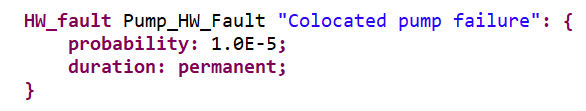
\includegraphics[width=.4\textwidth]{images/hw_fault2.png}
	\end{center}
	\vspace{-0.1in}
	\caption{Hardware Fault Definition}
	\label{fig:hwFault}
	%\vspace{-0.2in}
	%\vspace{-0.1in}
\end{figure}
\end{comment}
Users specify dependencies between the HW component faults and faults that are defined in other components, either HW or SW. The hardware fault then acts as a trigger for dependent faults. This allows a simple propagation from the faulty HW component to the SW components that rely on it, affecting the behavior on the outputs of the affected SW components. 
%\janet{An example is shown in Figure~\ref{fig:hwFaultProp}.}

\begin{comment}
\danielle{Consider leaving everything above and cutting what is left for explicit faults. It is just an example of the HW fault and some figures.}
%As an example, we will look yet again at the WBS. 
In the WBS example, assume that both the green and blue hydraulic pumps are located in the same compartment in the aircraft and an explosion in this compartment rendered both pumps inoperable.
%An accident took place and the green (normal) hydraulic pump took the force of an explosion. When the green hydraulic pump exploded, the pump shrapnel flew into the blue pump and it became from then on unoperable. 
The HW fault definition can be modeled first in the green hydraulic pump component as shown in Figure~\ref{fig:hwFault}. The activation of this fault triggers the activation of related faults as seen in the \textit{propagate\_to} statement shown below. % in Figure~\ref{fig:hwFaultProp}. 
Notice that these pumps need not be connected through a data port in order to specify this propagation. %Furthermore, the probability of the HW fault activation can be specified. 


\begin{figure}[h!]
	\vspace{-0.1in}
	\begin{center}
		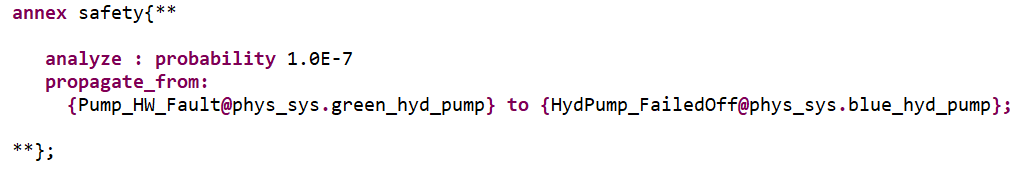
\includegraphics[width=.5\textwidth]{images/hw_prop_stmt.png}
	\end{center}
	\vspace{-0.1in}
	\caption{Hardware Fault Propagation Statement}
	\label{fig:hwFaultProp}
	%\vspace{-0.2in}
	%\vspace{-0.1in}
\end{figure}
\end{comment}

%The fault dependencies are specified in the system implementation where the system configuration that causes the dependencies becomes clear (e.g., binding between SW and HW components, co-location of HW components).

%This is because fault propagations are typically tied to the way components are connected or bound together; this information may not be available when faults are being specified for individual components. Having fault propagations specified outside of a component’s fault statements also makes it easier to reuse the component in different systems. 



\subsection{Fault Analysis Statements}
%An annotation in the AADL model determines the fault analysis statement (also referred to in this report as the fault hypothesis). This may specify either a maximum number of faults that can be active at any point in execution:
The Safety Annex also allows the user to specify constraints on the occurence of faults in the system.  
\begin{itemize}
\item The \emph{max fault hypothesis} specifies the maximum number of faults that can be active at any point in the analysis.  This is analogous to restricting the cutset to a specified maximum number of terms in the fault tree analysis in a traditional safety analysis.  
\item The \emph{probabilistic fault hypothesis} specifieds that only faults whose probability of simultaneous occurrence is above the given threshold should be onsidered.  This is analogous to restricting the cutsets to only those whose probability is above the specified value. 
\end{itemize}

%The fault analysis statement (also referred to as the fault hypothesis) resides in the AADL system implementation that is selected for verification. This may specify either a maximum number of faults that can be active at any point in execution.

\begin{comment}
\begin{figure}[h!]
	\vspace{-0.1in}
	%\begin{center}
		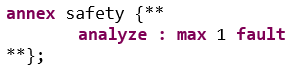
\includegraphics[width=0.4\textwidth]{images/hypothesisMaxN.png}
	%\end{center}
	\vspace{-0.1in}
	%%\caption{Max N Faults Analysis Statement}
	\label{fig:hypothesisMaxN}
\end{figure}
or that the only faults to be considered are those whose probability of simultaneous occurrence is above some probability threshold: 

\begin{figure}[h!]
	\vspace{-0.1in}
	%\begin{center}
		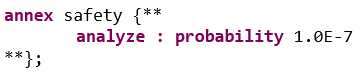
\includegraphics[width=0.5\textwidth]{images/hypothesisProb.png}
	%\end{center}
	\vspace{-0.1in}
	%\caption{Probability Analysis Statement}
	%\label{fig:hypothesisProb}
\end{figure}
\end{comment}
\noindent
In the former case, we assert that the sum of the true {\em fault\_\_trigger} variables is at or below some integer threshold.  In the latter, we determine all combinations of faults whose probabilities are above the specified probability threshold, and describe this as a proposition over {\em fault\_\_trigger} variables. 
%
\subsection{Fault Activation}
With the introduction of dependent faults, active faults are divided into two categories: independently active (activated by its own triggering event) and dependently active (activated when the faults they depend on become active). The top level fault hypothesis applies to independently active faults. Faulty behaviors augment nominal behaviors whenever their corresponding faults are active (either independently active or dependently active). 
%\janet{In addition, there is fault activation statement allowing users to access the activation status of specific faults so they can be used in property specifications, such as to describe a failing or non failing component.}











\section{Tool Architecture and Implementation}
\label{sec:implementation}

The Safety Annex is written in Java as a plug-in for the OSATE AADL toolset, which is built on Eclipse.  It is not designed as a stand-alone extension of the language, but works with behavioral contracts specified using the AGREE AADL annex~\cite{NFM2012:CoGaMiWhLaLu}. 
The architecture of the Safety Annex is shown in Figure~\ref{fig:plugin-arch}.

\begin{figure}
	\begin{center}
		%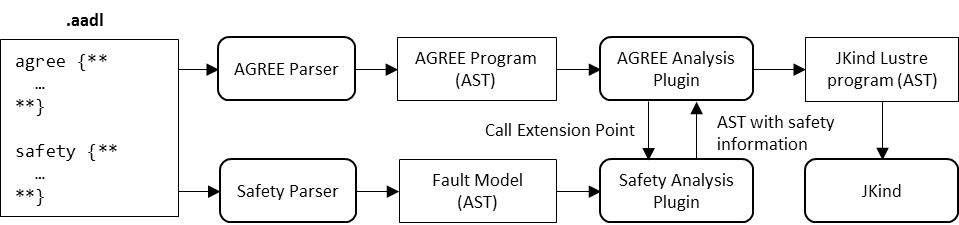
\includegraphics[trim=0 400 430 0,clip,width=0.85\textwidth]{images/arch.png}
		\includegraphics[width=\columnwidth]%.5\dimexpr\textwidth-2cm\relax]
	{images/arch.png}
	\end{center}
	\vspace{-0.2in}
	\caption{Safety Annex Plug-in Architecture}
	\label{fig:plugin-arch}
	\vspace{-0.2in}
\end{figure}

AGREE contracts are used to define the nominal behaviors of system components as {\em guarantees} that hold when {\em assumptions} about the values the component's environment are met. When an AADL model is annotated with AGREE contracts and the fault model is created using the Safety Annex, the model is transformed through AGREE into a Lustre model~\cite{Halbwachs91:IEEE} containing the behavioral extensions defined in the AGREE contracts for each system component. 

%This program is intercepted by the Safety Annex plugin and fault model information is added in two ways, depending on which form of fault analysis is being run. 

%\subsection{Verification in the Presence of Faults}
When performing fault analysis, the Safety Annex extends the AGREE contracts to allow faults to modify the behavior of component inputs and outputs. An example of a portion of an initial AGREE node and its extended contract is shown in Figure~\ref{fig:lustre}. The left column of the figure shows the nominal Lustre pump definition is shown with an AGREE contract on the output; and the right column shows the additional local variables for the fault (boxes 1 and 2), the assertion binding the fault value to the nominal value (boxes 3 and 4), and the fault node definition (box 5). Once augmented with fault information, the AGREE model (translated into the Lustre dataflow language~\cite{Halbwachs91:IEEE}) follows the standard translation path to the model checker JKind~\cite{2017arXiv171201222G}, an infinite-state model checker for safety properties. 

\begin{figure}[h!]
	\hspace*{-2cm}
	%\vspace{-0.3in} 
	\begin{center}
		%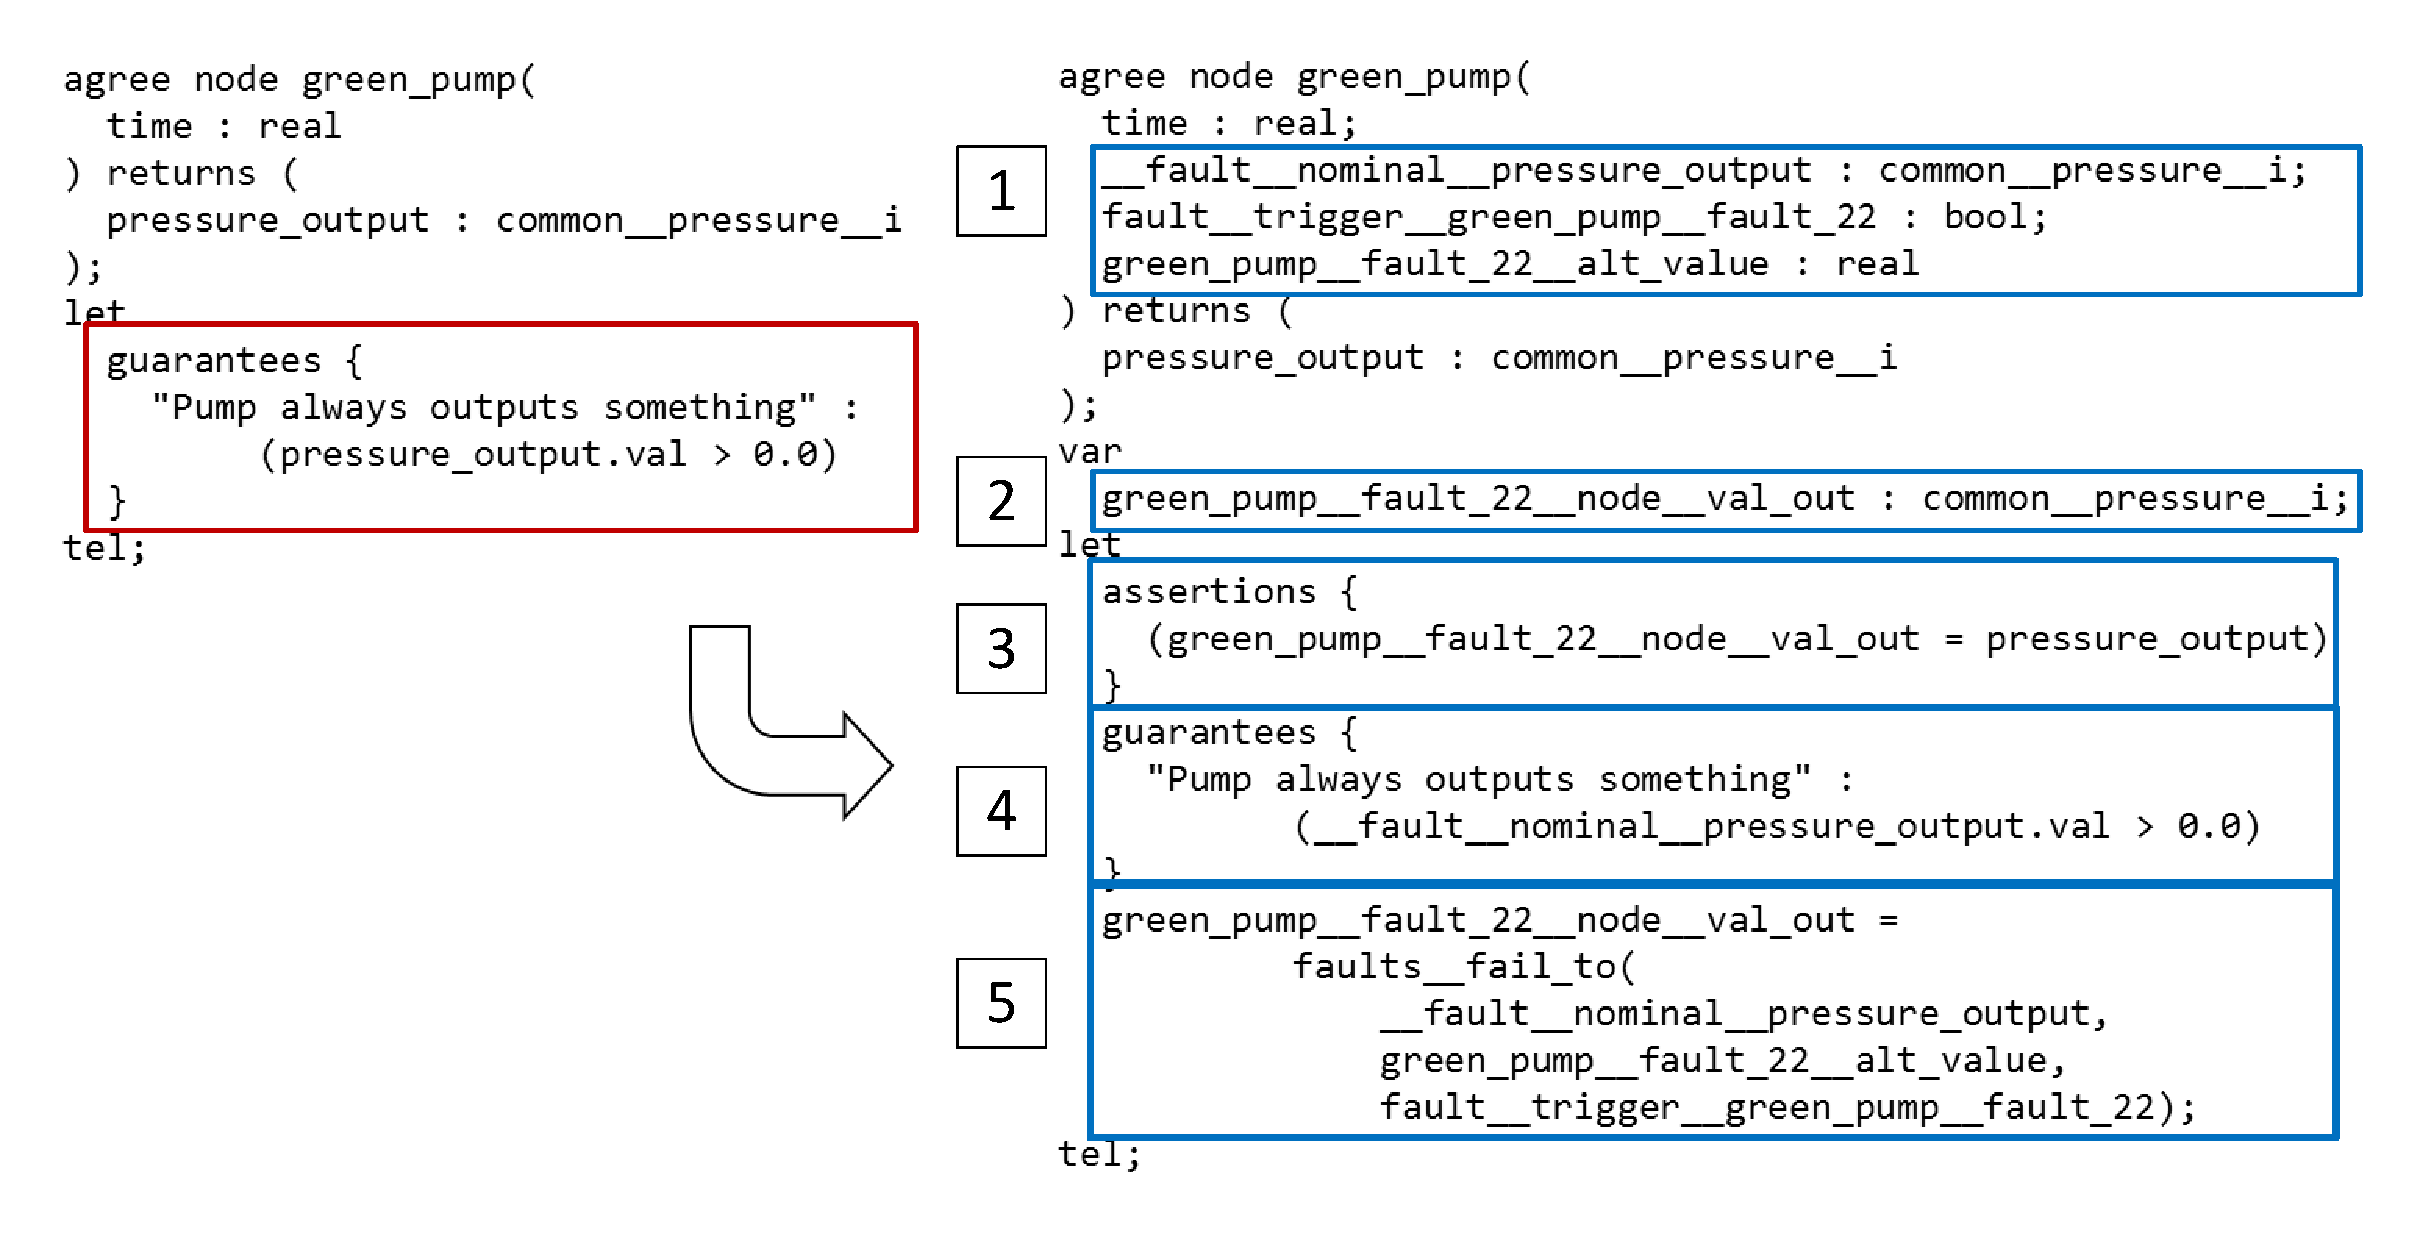
\includegraphics[trim=0 690 -10 70,clip,width=1.5\dimexpr\textwidth-2cm\relax]{images/lustre.pdf}
		\includegraphics[width=\columnwidth]%.5\dimexpr\textwidth-2cm\relax]
	{images/lustre.jpg}
		%\caption{Nominal AGREE node and its extension with faults}
		\caption{Nominal AGREE Node and Extension with Faults}
		\label{fig:lustre}
	\end{center}
	%\vspace{-0.3in}
\end{figure}

There are two different types of fault analysis that can be performed on a fault model. The Safety Annex plugin intercepts the AGREE program and add fault model information to the model depending on which form of fault analysis is being run.

\textbf{Verification in the Presence of Faults}: This analysis returns one counterexample when fault activation per the fault hypothesis can cause violation of a property. The augmentation from Safety Annex to the AGREE program includes traceability information so that when counterexamples are displayed to users, the active faults for each component are visualized.

\textbf{Generate Minimal Cut Sets}: This analysis returns all minimal cut sets that lead to the violation of a property, transformed from a full enumeration of all minimal set of model elements necessary for the inductive proofs of the property~\cite{Ghassabani2017EfficientGO,bendik2018online}.
\begin{comment}
\danielle{We will have to discuss this subsection. As is, it is not complete or sufficient for a full description, but I am not sure we want a full description since this stuff isn't published yet.} This analysis collects all minimal set of fault combinations that can cause violation of a property.
%\subsection{Generate Minimal Cut Sets}
Given a complex model, it is often useful to extract traceability information related to the proof, in other words, which portions of the model were necessary to construct the proof. An algorithm was introduced by Ghassabani, et. al. to provide Inductive Validity Cores (IVCs) as a way to determine which model elements are necessary for the inductive proofs of the safety properties for sequential systems~\cite{GhassabaniGW16}. Given a safety property of the system, a model checker can be invoked in order to construct a proof of the property. The IVC generation algorithm extracts traceability information from the proof process and returns a minimal set of the model elements required in order to prove the property. Later research extended this algorithm in order to produce all Minimal Inductive Validity Cores (All-MIVCs) to provide a full enumeration of all minimal set of model elements necessary for the inductive proofs of a safety property~\cite{Ghassabani2017EfficientGO}. 
\end{comment}



\begin{comment}
The IVC algorithm considers a constraint system consisting of the assumptions and contracts of system components and the negation of the safety property of interest (i.e. the top level event). It then collects what are called Minimal Unsatisfiable Subsets (MUSs) of this constraint system; these are the minimal explanations of the constraint systems infeasibility in terms of the \textit{negation} of the safety property. Equivalently, these are the minimal model elements necessary to proof the safety property. In section \ref{sec:definitions}, we show the formal definitions of IVCs in detail. 

In order to compositionally generate minimal cut sets, the all IVC algorithm is used~\cite{Ghassabani2017EfficientGO}, but instead of annotating the model with IVC elements consisting of only assumptions and contracts, we insert the faults in each layer constrained to false. The leaf nodes contribute only constrained faults to the IVC elements as shown in Figure~\ref{fig:ivcElements1}. 
\end{comment}
\begin{comment}
In this approach, we use the all MIVCs algorithm to consider a constraint system consisting of the negation of the top level safety property, the contracts of system components, as well as the faults in each layer constrained to false. It then collects what are called Minimal Unsatisfiable Subsets (MUSs) of this constraint system; these are the minimal explanations of the constraint systems infeasibility in terms of the \textit{negation} of the safety property. Equivalently, these are the minimal model elements necessary to proof the safety property. In section \ref{sec:definitions}, we show the formal definitions in detail. The leaf nodes contribute only constrained faults to the IVC elements as shown in Figure~\ref{fig:ivcElements1}. 

In the non-leaf layers of the program, both contracts and constrained faults are considered as shown in Figure~\ref{fig:ivcElements2}. The reason for this is that the contracts are used to prove the properties at the next highest level and are necessary for the verification of the properties. 

The all MIVCs algorithm returns the minimal set of these elements necessary to prove the properties. This equates to any contracts or inactive faults that must be present in order for the verification of properties in the model. From here, we perform a number of algorithms to transform all MIVCs into minimal cut sets (see Section~\ref{sec:theory} for more details on the transformation algorithms).
\end{comment}
\begin{comment}
\begin{figure}[h!]
	\hspace*{-2cm}
	\vspace{-0.1in} 
	\begin{center}
		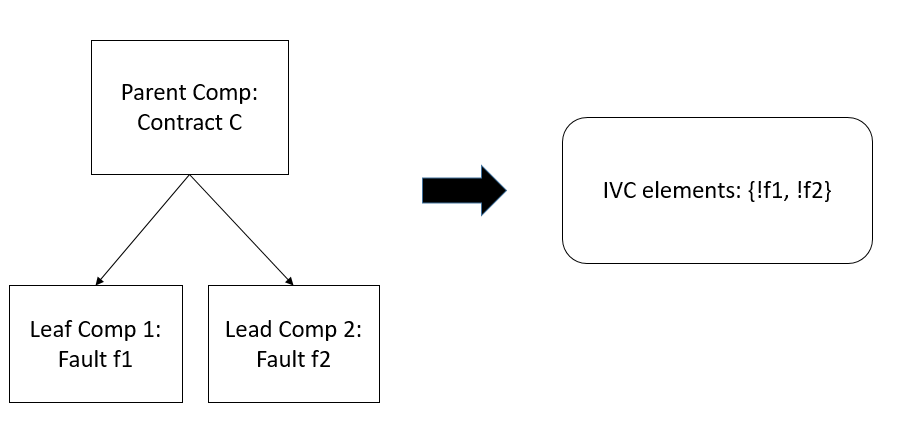
\includegraphics[scale=0.5]{images/ivcElements1.png}
	\caption{IVC Elements used for Consideration in a Leaf Layer of a System}
		\label{fig:ivcElements1}
	\end{center}
\end{figure}

\begin{figure}[h!]
	\hspace*{-2cm}
	\vspace{-0.1in} 
	\begin{center}
		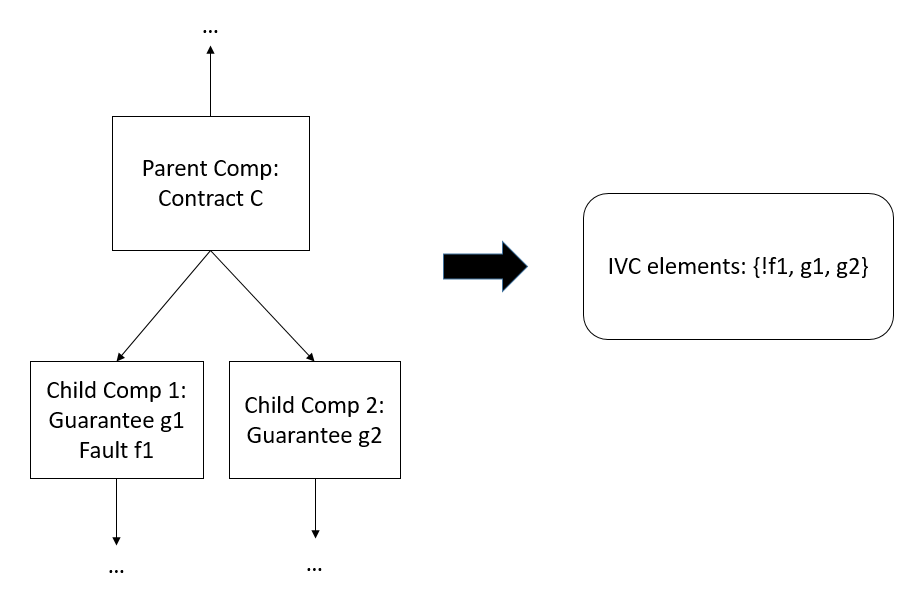
\includegraphics[scale=0.5]{images/ivcElements2.png}
	\caption{IVC Elements used for Consideration in a Middle Layer of a System}
		\label{fig:ivcElements2}
	\end{center}
\end{figure}
\end{comment}

\begin{comment}
The architecture of the Safety Annex is shown in Figure~\ref{fig:plugin-arch}.  It is written in Java as a plug-in for the OSATE AADL toolset, which is built on Eclipse.  It is not designed as a stand-alone extension of the language, but works with behavioral contracts specified in AGREE AADL annex and associated tools~\cite{NFM2012:CoGaMiWhLaLu}.  AGREE allows {\em assume-guarantee} behavioral contracts to be added to AADL components.  The language used for contract specification is based on the Lustre dataflow language~\cite{Halbwachs91:IEEE}. AGREE improves scalability of formal verification to large systems by decomposing the analysis of a complex system architecture into a collection of smaller verification tasks that correspond to the structure of the architecture.

\begin{figure}
	\begin{center}
		%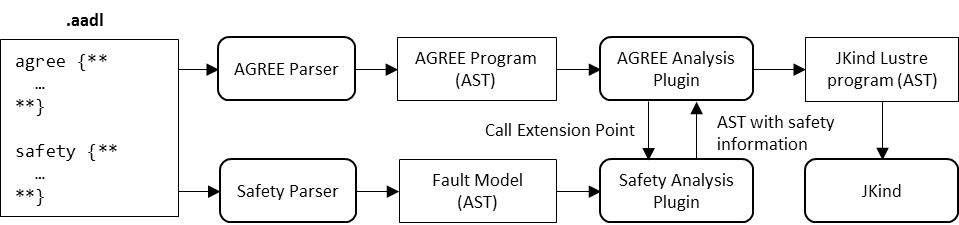
\includegraphics[trim=0 400 430 0,clip,width=0.85\textwidth]{images/arch.png}
		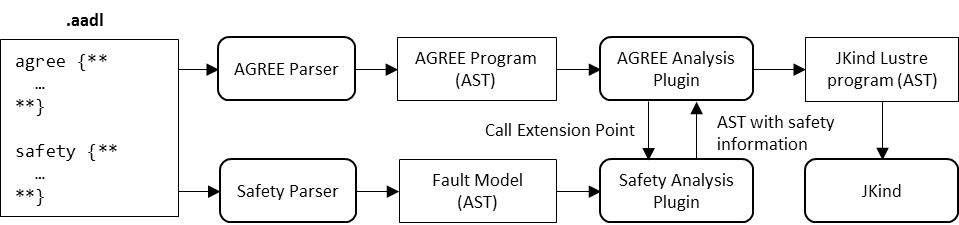
\includegraphics[width=.9\textwidth]{images/arch.png}
	\end{center}
	\vspace{-0.2in}
	\caption{Safety Annex Plug-in Architecture}
	\label{fig:plugin-arch}
\end{figure}

AGREE contracts are used to define the nominal behaviors of system components as {\em guarantees} that hold when {\em assumptions} about the values the component's environment are met.  The Safety Annex extends these contracts to allow faults to modify the behavior of component inputs and outputs.  To support these extensions, AGREE implements an Eclipse extension point interface that allows other plug-ins to modify the generated abstract syntax tree (AST) prior to its submission to the solver.  If the Safety Annex is enabled, these faults are added to the AGREE contract and, when triggered, override the nominal guarantees provided by the component.  

An example of a portion of an initial AGREE node and its extended contract is shown in Figure~\ref{fig:lustre}. 
In the left column of the figure, the nominal Lustre pump definition is shown with an AGREE contract on the output. In the right column, the additional local variables for the fault are seen in boxes 1 and 2, the assertion binding the fault value to the nominal value is seen in boxes 3 and 4, and the fault node definition is given in box 5. 

\begin{figure}[h!]
	\hspace*{-2cm}
	\vspace{-0.3in} 
	\begin{center}
		%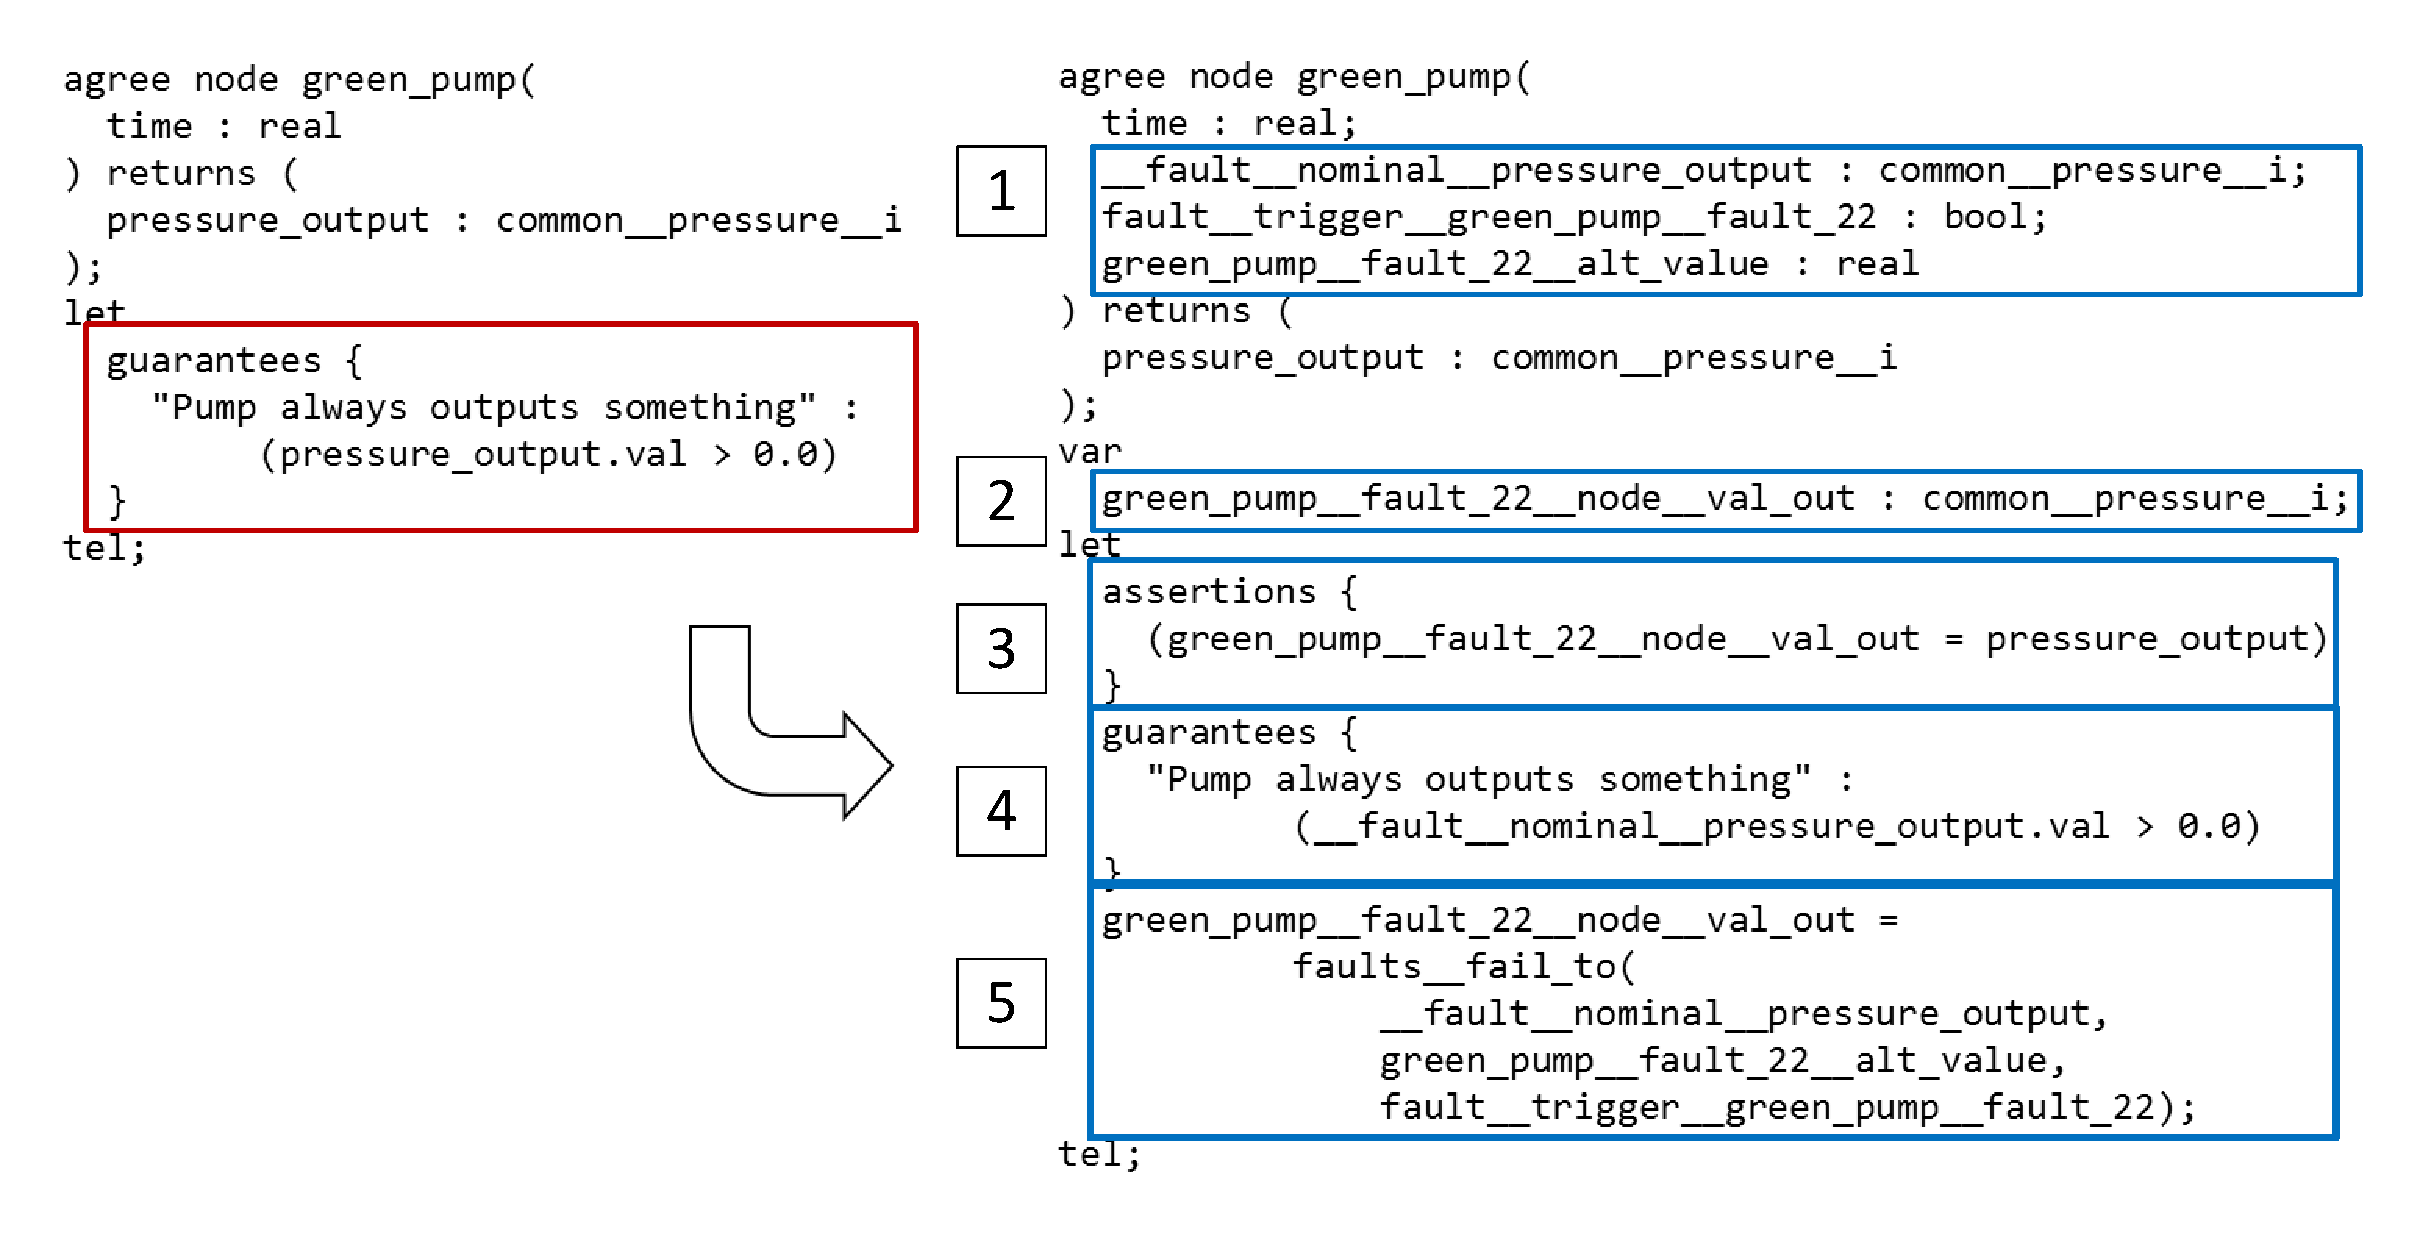
\includegraphics[trim=0 690 -10 70,clip,width=1.5\dimexpr\textwidth-2cm\relax]{images/lustre.pdf}
		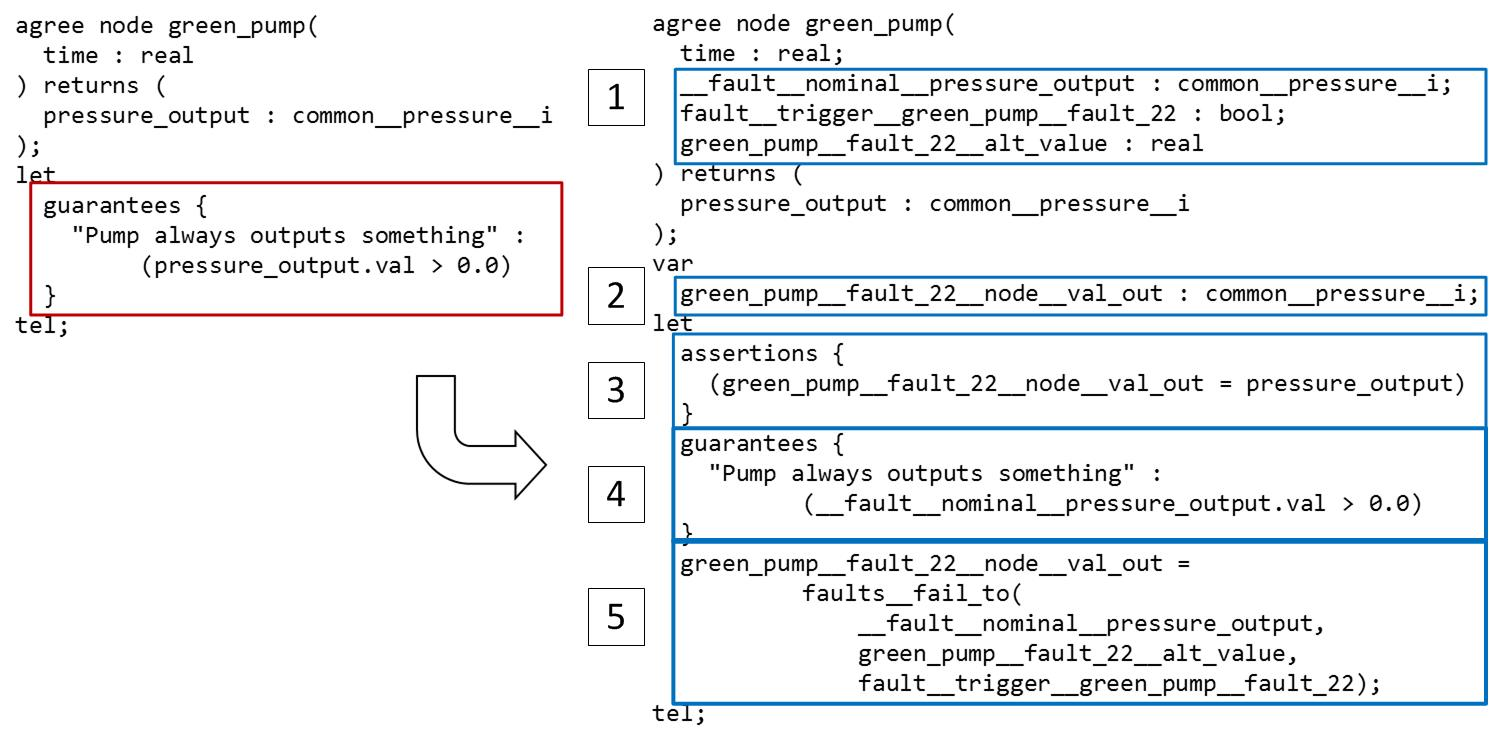
\includegraphics[scale=0.3]{images/lustre.jpg}
		\caption{Nominal AGREE node and its extension with faults}
		\label{fig:lustre}
	\end{center}
	\vspace{-0.3in}
\end{figure}


Once augmented with fault information, the AGREE model follows the standard translation path to the model checker JKind~\cite{2017arXiv171201222G}, an infinite-state model checker for safety properties.  The augmentation includes traceability information so that when counterexamples are displayed to users, the active faults for each component are visualized.

The architecture of the Safety Annex is shown in Figure~\ref{fig:plugin-arch}.  It is written in Java as a plug-in for the OSATE AADL toolset, which is built on Eclipse.  It is not designed as a stand-alone extension of the language, but works with behavioral contracts specified in AGREE AADL annex and associated tools~\cite{NFM2012:CoGaMiWhLaLu}.  AGREE allows {\em assume-guarantee} behavioral contracts to be added to AADL components.  The language used for contract specification is based on the Lustre dataflow language~\cite{Halbwachs91:IEEE}. AGREE improves scalability of formal verification to large systems by decomposing the analysis of a complex system architecture into a collection of smaller verification tasks that correspond to the structure of the architecture.

\begin{figure}
	\begin{center}
		%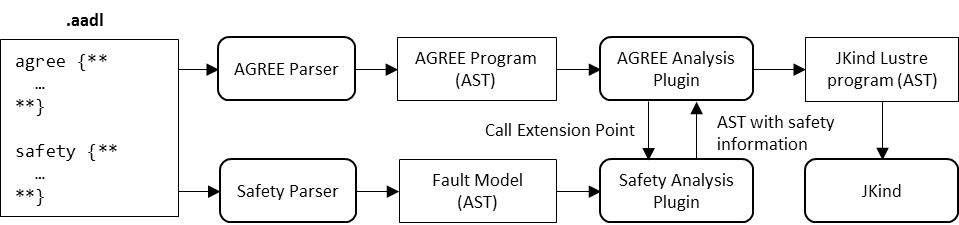
\includegraphics[trim=0 400 430 0,clip,width=0.85\textwidth]{images/arch.png}
		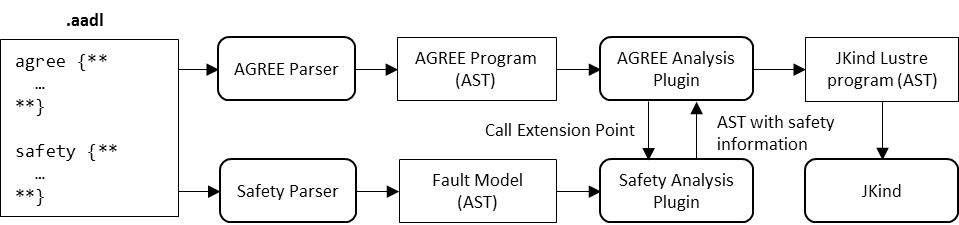
\includegraphics[width=.9\textwidth]{images/arch.png}
	\end{center}
	\vspace{-0.2in}
	\caption{Safety Annex Plug-in Architecture}
	\label{fig:plugin-arch}
\end{figure}

AGREE contracts are used to define the nominal behaviors of system components as {\em guarantees} that hold when {\em assumptions} about the values the component's environment are met.  The Safety Annex extends these contracts to allow faults to modify the behavior of component inputs and outputs.  To support these extensions, AGREE implements an Eclipse extension point interface that allows other plug-ins to modify the generated abstract syntax tree (AST) prior to its submission to the solver.  If the Safety Annex is enabled, these faults are added to the AGREE contract and, when triggered, override the nominal guarantees provided by the component.  

An example of a portion of an initial AGREE node and its extended contract is shown in Figure~\ref{fig:lustre}.  %The \texttt{\_\_fault} variables and declarations are added to allow the contract to override the nominal behavioral constraints (provided by guarantees) on outputs.  In the Lustre language, \texttt{assertion}s are constraints that are assumed to hold in the transition system. 
In the left column of the figure, the nominal Lustre pump definition is shown with an AGREE contract on the output. In the right column, the additional local variables for the fault are seen in boxes 1 and 2, the assertion binding the fault value to the nominal value is seen in boxes 3 and 4, and the fault node definition is given in box 5. 

%A  benefit of utilizing the AGREE behavioral annex is the ability to perform both monolithic and compositional analysis on the nominal model. AGREE allows {\em assume-guarantee} behavioral contracts to be added to AADL components.  The language used for contract specification is based on the Lustre dataflow language~\cite{Halbwachs91:IEEE} and the nominal model (AADL model annotated with AGREE contracts) is translated into Lustre before being sent to the JKind model checker for verification\cite{2017arXiv171201222G}. 

%When a user selects to run the fault analysis during verification, the AGREE contracts are automatically extended in Lustre in order to allow faults to modify the behavior of component outputs. These injections into the Lustre model are shown in Figure~\ref{fig:lustre}. 

\begin{figure}[h!]
	\hspace*{-2cm}
	\vspace{-0.3in} 
	\begin{center}
		%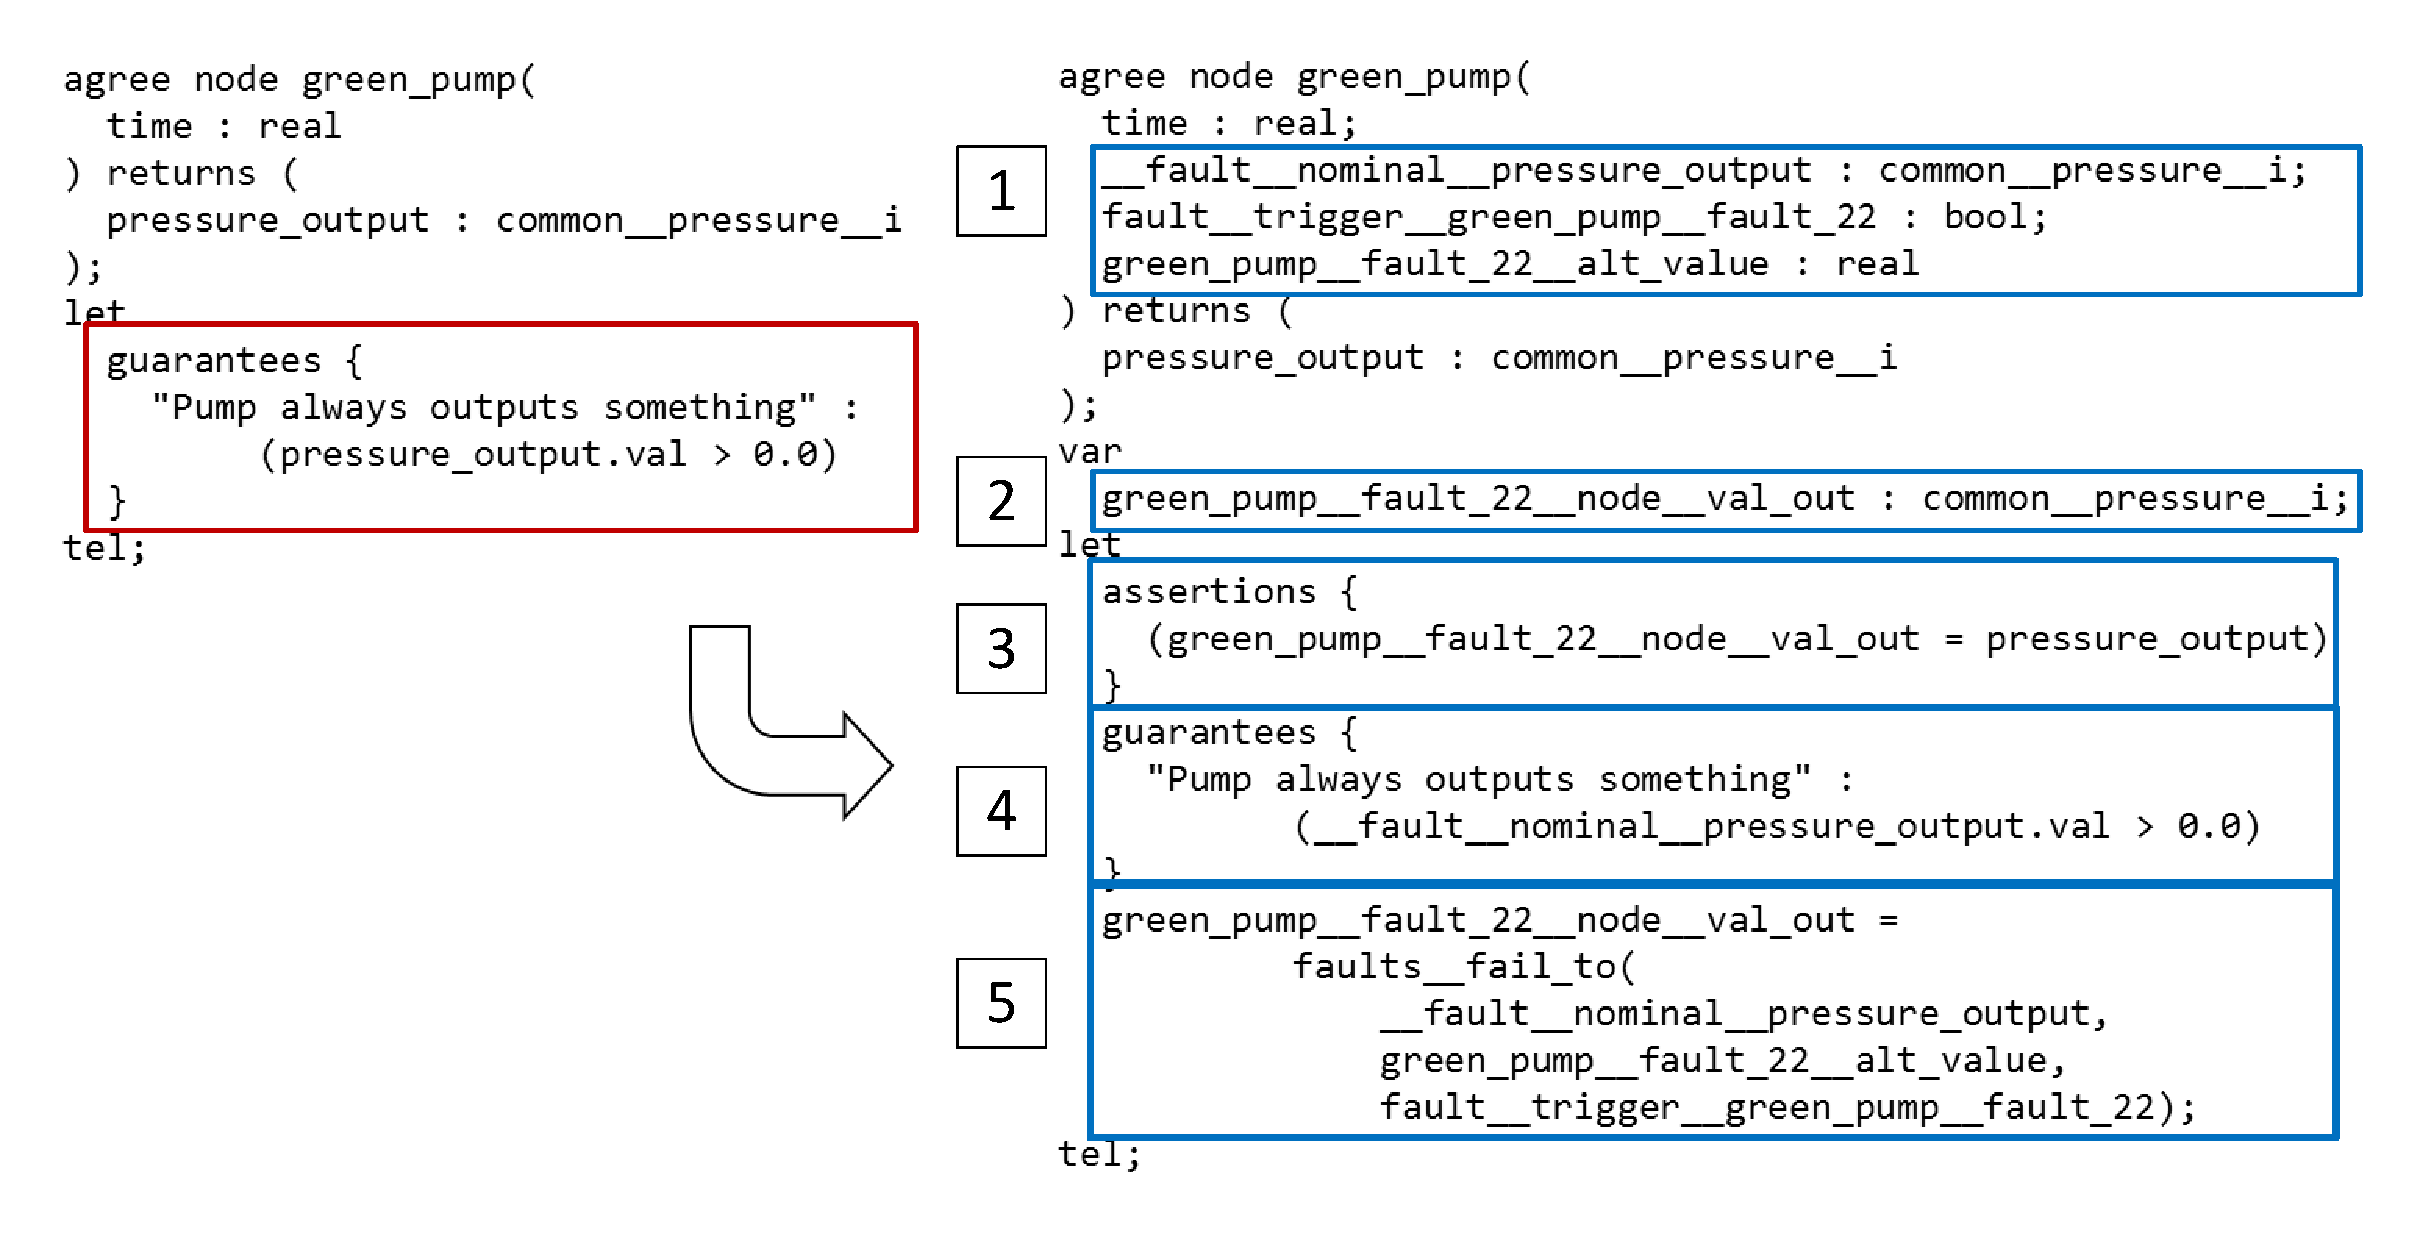
\includegraphics[trim=0 690 -10 70,clip,width=1.5\dimexpr\textwidth-2cm\relax]{images/lustre.pdf}
		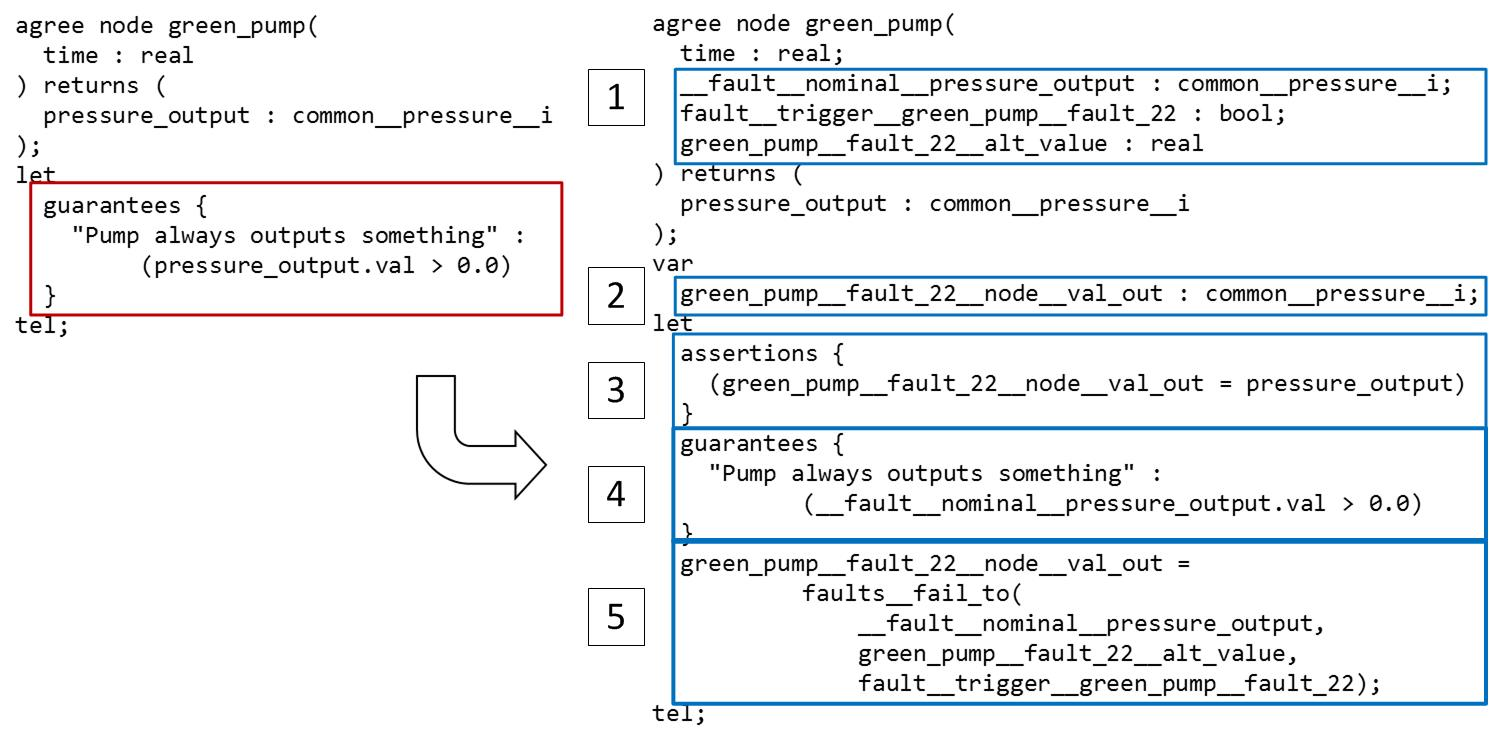
\includegraphics[scale=0.3]{images/lustre.jpg}
		\caption{Nominal AGREE node and its extension with faults}
		\label{fig:lustre}
	\end{center}
	\vspace{-0.3in}
\end{figure}

\begin{comment}
\begin{figure}
	\vspace{-0.1in}
	%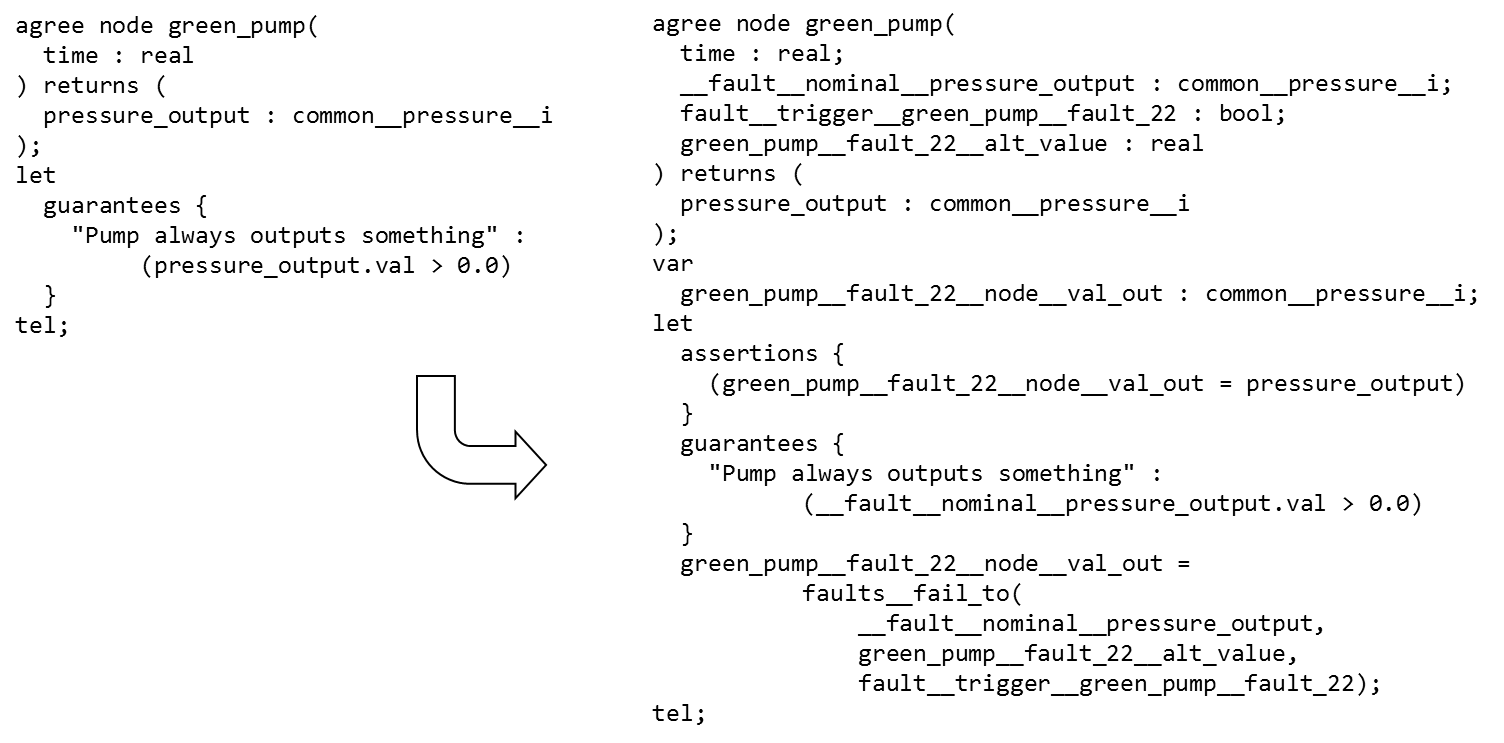
\includegraphics[trim=30 150 120 10,clip,width=\textwidth]{images/sample_code.png}
	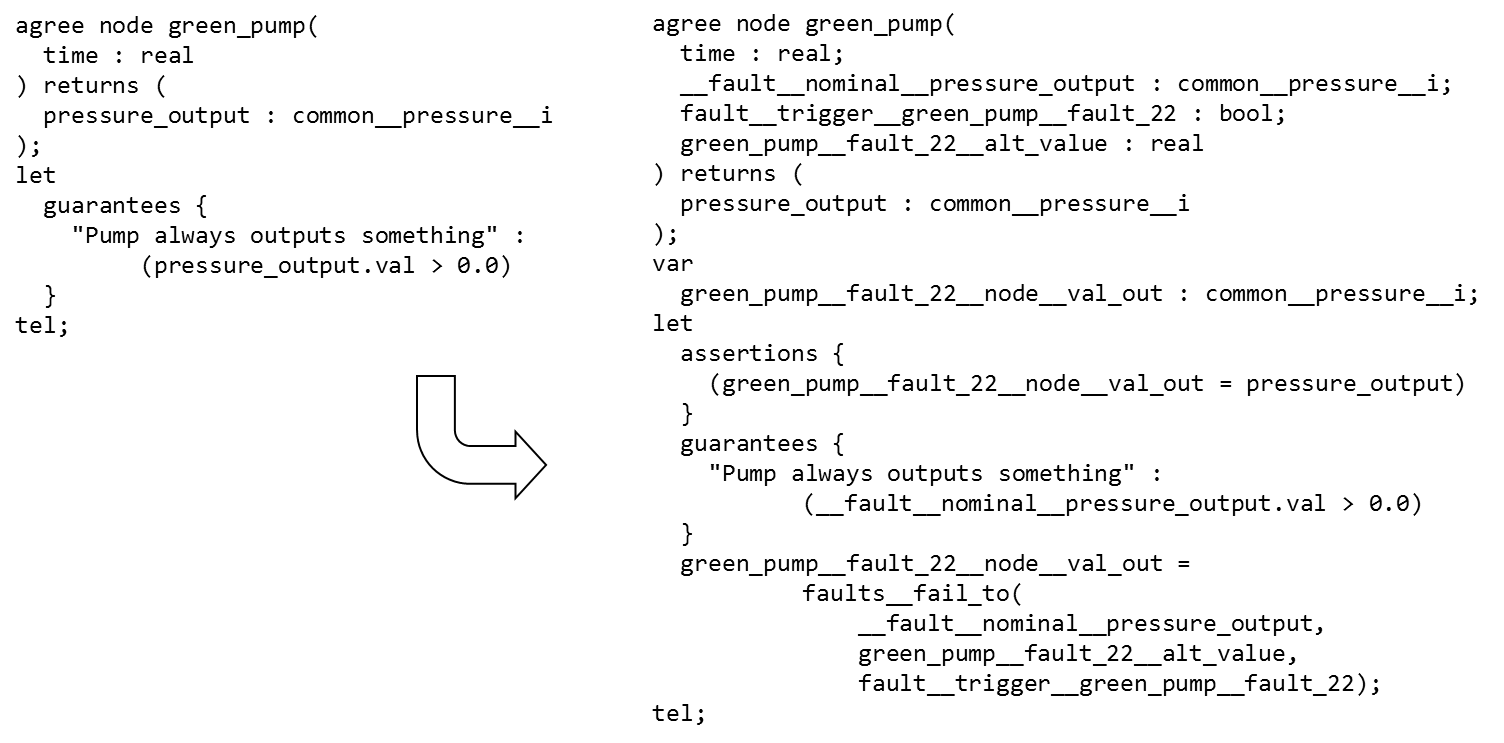
\includegraphics[width=\textwidth]{images/sample_code.png}
	\vspace{-0.3in}
	\caption{Nominal AGREE node and its extension with faults}
	\label{fig:comp}
\end{figure}
\end{comment}
%An annotation in the AADL model determines the fault hypothesis.  This may specify either a maximum number of faults that can be active at any point in execution (typically one or two), or that only faults whose probability of simultaneous occurrence is above some probability threshold should be considered. In the former case, we assert that the sum of the true {\em fault\_\_trigger} variables is below some integer threshold.  In the latter, we determine all combinations of faults whose probabilities are above the specified probability threshold, and describe this as a proposition over {\em fault\_\_trigger} variables.
%
%With the introduction of dependent faults, active faults are divided into two categories: independently active (activated by its own triggering event) and dependently active (activated when the faults they depend on become active). The top level fault hypothesis applies to independently active faults. Faulty behaviors augment nominal behaviors whenever their corresponding faults are active (either independently active or dependently active).

%Once augmented with fault information, the AGREE model follows the standard translation path to the model checker JKind~\cite{2017arXiv171201222G}, an infinite-state model checker for safety properties.  The augmentation includes traceability information so that when counterexamples are displayed to users, the active faults for each component are visualized.


%For fault analysis, we separate the possible analyses available to users into two distinct actions and describe them here.


\section{Analysis of the Model}
\label{sec:fault_analysis_2}
In this section we describe results from the nominal model analysis and the fault analysis.  

\subsection{Nominal Model Analysis}
Before performing fault analysis, users should first check that the safety properties are satisfied by the nominal design model. This analysis can be performed monolithically or compositionally in AGREE. Using monolithic analysis, the contracts at the lower levels of the architecture are flattened and used in the proof of the top level safety properties of the system. Compositional analysis, on the other hand, will perform the proof layer by layer top down, essentially breaking the larger proof into subsets of smaller problems. For a more comprehensive description of these types of proofs and analyses, see additional publications related to AGREE \cite{cofer2012compositional,QFCS15:backes} 

The WBS has a total of 13 safety properties at the top level that are supported by subcomponent assumptions and guarantees. These are shown in Table \ref{tab:safetyProperties}. Given that there are 8 wheels, contract S18-WBS-0325-wheelX is repeated 8 times, one for each wheel. The behavioral model in total consists of 36 assumptions and 246 supporting guarantees.

\begin{table}[]
\begin{tabular}{@{}ll}
\toprule
\textbf{S18-WBS-R-0321} \\Loss of all wheel braking during landing or RTO shall be less than $5.0 \times 10^{-7}$ per flight.                                    \\ \midrule 
\textbf{S18-WBS-R/L-0322}  \\ Asymmetrical loss of wheel braking (Left/Right) shall be less than $5.0 \times 10^{-7}$ per flight. \\ \midrule
\textbf{S18-WBS-0323} \\ Never inadvertent braking with all wheels locked shall be less than $1.0 \times 10^{-9}$ per takeoff.                                                                                                                                                                                                               \\ \midrule
\textbf{S18-WBS-0324}  \\ Never inadvertent braking with all wheels shall be less than $1.0 \times 10^{-9}$ per takeoff.                                                                                                            \\ \midrule
\textbf{S18-WBS-0325-wheelX} \\ Never inadvertent braking of wheel X shall be less than $1.0 \times 10^{-9}$ per takeoff.                                                                                                           .                                                                                                                 \\ \bottomrule
\end{tabular}
\caption{Safety Properties of WBS}
\label{tab:safetyProperties}
\end{table}  

\subsection{Fault Model Analysis}
There are two main options for fault model analysis using the Safety Annex. The first option injects faulty behavior allowed by faulty hypothesis into the AGREE model and returns this model to JKind for analysis. This allows for the activity of faults within the model and traceability information provides a way for users to view a counterexample to a violated contract in the presence of faults. The second option is used to generate minimal cut sets for the model. The model is annotated with fault activation that are constrained to false as well as intermediate level guarantees as model elements for consideration for the all Minimal Inductive Validity Cores (All-MIVCs)
algorithm. The All-MIVCs traces the minimal set of model elements used to produce minimal cut sets and is described in Section~\ref{sec:theory}. This subsection presents these options and discusses the analytical results obtained. 

\subsubsection{Verification in the Presence of Faults: Max N Analysis}
Using a max number of faults for the hypothesis, the user can constrain the number of simultaneously active faults in the model. The faults are added to the AGREE model for the verification. Given the constraint on the number of possible simultaneously active faults, the model checker attempts to prove the top level properties given these constraints. If this cannot be done, the counterexample provided will show which of the faults (N or less) are active and which contracts are violated. 

The user can choose to perform either compositional or monolithic analysis using a max N fault hypothesis. In compositional analysis, the analysis proceeds in a top down fashion. To prove the top level properties, the properties in the layer directly beneath the top level are used to perform the proof. The analysis proceeds in this manner. Users constrain the maximum number of faults within each layer of the model by specifying the maximum fault hypothesis statement to that layer. If any lower level property failed due to activation of faults, the property verification at the higher level can no longer be trusted because the higher level properties were proved based on the assumption that the direct sub-level contracts are valid. This form of analysis is helpful to see weaknesses in a given layer of the system. 

In monolithic analysis the layers of the model are flattened, which allows a direct correspondence between all faults in the model and their effects on the top level properties. As with compositional analysis, a counterexample shows these N or less active faults. 

\subsubsection{Verification in the Presence of Faults: Probabilistic Analysis} 
Given a probabilistic fault hypothesis, this corresponds to performing analysis with the combinations of faults whose occurrence probability is less than the probability threshold. This is done by inserting assertions that allow those combinations in the Lustre code. If the model checker proves that the safety properties can be violated with any of those combinations, one of such combination will be shown in the counterexample. 

Probabilistic analysis done in this way must utilize the monolithic AGREE option. For compositional probabilistic analysis, see Section~\ref{sec:prob_generate}.

To perform this analysis, it is assumed that the non-hardware faults occur independently and possible combinations of faults are computed and passed to the Lustre model to be checked by the model checker. As seen in Algorithm 1, the computation first removes all faults from consideration that are too unlikely given the probability threshold. The remaining faults are arranged in a priority queue $\mathcal{Q}$ from high to low. Assuming independence in the set of faults, we take a fault with highest probability from the queue (step 5) and attempt to combine the remainder of the faults in $\mathcal{R}$ (step 7). If this combination is lower than the threshold (step 8), then we do not take into consideration this set of faults and instead remove the tail of the remaining faults in $\mathcal{R}$. 
 
\begin{algorithm}[H]
	% \KwData{this text}
	% \KwResult{how to write algorithm with \LaTeX2e }
	$\mathcal{F} = \{\}$ : fault combinations above threshold \;
	$\mathcal{Q}$ : faults, $q_i$, arranged with probability high to low \;
	$\mathcal{R} = \mathcal{Q}$ , with $r \in \mathcal{R}$\;
	\While{$\mathcal{Q} \neq \{\} \land \mathcal{R} \neq \{\}$ }{
		$q =$ removeTopElement($\mathcal{Q}$) \;
		\For{$i=0:|\mathcal{R}|$}{
			$prob = q \times r_i$ \;
			\eIf{prob $<$ threshold}{
				removeTail($\mathcal{R}, j=i:|\mathcal{R}|$)\;
			}{
				add($\{q, r_i\}, \mathcal{Q}$)\;
				add($\{q, r_i\}, \mathcal{F}$)\;
			} % end if else
		} % end for
	} % end while
	\caption{Monolithic Probability Analysis}
	\label{alg:prob_monolithic}
\end{algorithm}
In this calculation, we assume independence among the faults, but in the Safety Annex it is possible to define dependence between faults using a fault propagation statement. After fault combinations are computed using Algorithm~\ref{alg:prob_monolithic}, the triggered dependent HW faults are added to the combination as appropriate. The dependencies are implemented in the \textit{Verify in the Presence of Faults} options for analysis, but not yet implemented in the \textit{Generate Minimal Cut Sets} analysis options.

\subsubsection{Generate Minimal Cut Sets: Max N Analysis}
\label{sec:maxN_generate}
As described in Section~\ref{sec:implementation}, \textit{Generate Minimal Cut Sets} analysis uses the All-MIVCs algorithm to provide a full enumeration of all minimal set of model elements necessary for the proof of each top-level safety property in the model, and then transforms all MIVCs into all minimal cut sets. In Max N analysis, the minimal cut sets are pruned to include only those with at cardinality less or equal to the max N number specified in the fault hypothesis and displayed to the user.

Generate MinCutSet analysis was performed on the Wheel Brake System and results are shown in Table~\ref{tab:wbs_maxN_results}. Notice in Table~\ref{tab:wbs_maxN_results}, the label across the top row refers to the cardinality (C) and how many cut sets of that cardinality. When the analysis is run, the user specifies the value N. This gives cut sets of cardinality \textit{less than or equal to} N. (For the full text of the properties, see Table~\ref{tab:safetyProperties}.)

\begin{center}
\begin{table}[h]
    \begin{tabular}{ | l | l | l | l | l | l | l | l |}
    \hline
    \textbf{Property} & $\bm{c = 1}$ & $\bm{c = 2}$ & $\bm{c = 3}$ & $\bm{c = 4}$ 
		& $\bm{c = 5}$ & $\bm{c = 6}$ & $\bm{c = 7+}$  \\ \hline \hline
    R-0321 & 6 & 0 & 0 & 1& 144&7776 &- \\ \hline
    R-0322 & 32 & 0 & 0 &0 &0 &0 &- \\ \hline
    L-0322 & 32 & 0 & 0 &0 &0 &0 &- \\ \hline
    0323 & 90 & 0 & 0 &0 &0 &0 &- \\ \hline
    0324 & 8 & 3,401 & 6,800 &66,472 & 435,358&1,892,832 &- \\ \hline
    0325-WX & 20 & 0 & 0 &0 &0 & 0&- \\ \hline
    \end{tabular}
    \caption{WBS MinCutSet Analysis Results for Cardinality $c$}
    \label{tab:wbs_maxN_results}
\end{table}
\end{center}



Due to the increasing number of possible fault combinations at $N=6$, the computational time increases quickly. The WBS analysis was only run to $N=6$ for this reason. 

\subsubsection{Generate Minimal Cut Sets: Probabilistic Analysis}
\label{sec:prob_generate}
Both probabilistic analysis and max N analysis use the same minimal cut set generation algorithm, except that in probabilistic analysis, the minimal cut sets are pruned to include only those fault combinations whose probability of simultaneous occurrence exceed the given threshold in the probability hypothesis. Note that with probablistic hypothesis, \textit{Verify in the Presence of Faults} is performed using only monolithic analysis, but generating minimal cut sets is performed using compositional analysis.


The probabilistic analysis for the WBS was given a top level threshold of $1.0 \times 10^{-9}$ as stated in AIR6110. The faults associated with various components were all given probability of occurrence compatible with the discussion in this same document. 

As shown in Table~\ref{tab:wbs_prob_results}, the number of allowable combinations drops considerably when given probabilistic threshold as compared to just fault combinations of certain cardinalities. For example, one contract (inadvertent wheel braking of all wheels) had over a million minimal cut sets produced when looking at it in terms of max N analysis, but after taking probabilities into account, it is seen that only one combination of faults can violate this property. (For the full text of the properties, see Table~\ref{tab:safetyProperties}.)

\begin{center}
\begin{table}[h]
    \begin{tabular}{ | l | l | l | l | l | l | l | l | l |}
    \hline
    \textbf{Property} & $\bm{c = 1}$ & $\bm{c = 2}$ & $\bm{c = 3}$ & $\bm{c = 4}$ 
		& $\bm{c = 5}$ & $\bm{c = 6}$ & $\bm{c = 7}$ & $\bm{c = 8}$  \\ \hline \hline
    R-0321 & 0 & 0 & 0 & 0 & 0 & 0 & 0 & 0 \\ \hline
    R-0322 & 32 & 0 & 0 &0 &0 &0 &0& 0  \\ \hline
    L-0322 & 32 & 0 & 0 & 0 & 0 & 0 & 0 & 0  \\ \hline
    0323 & 90 & 0 & 0 & 0 & 0 & 0 & 0 & 0  \\ \hline
    0324 & 0 & 1 & 0 & 0 & 0 & 0 & 0 & 0  \\ \hline
    0325-WX & 20 & 0 & 0 &0 &0 & 0 & 0 & 0  \\ \hline
    \end{tabular}
    \caption{WBS MinCutSet Results for Probabilistic Analysis}
    \label{tab:wbs_prob_results}
\end{table}
\end{center}

\subsubsection{Results from Generate Minimal Cut Sets}
Results from Generate Minimal Cut Sets analysis can be represented in one of the following forms.
\begin{enumerate}
\item The minimal cut sets can be presented in text form with the total number per property, cardinality of each, and description strings showing the property and fault information. A sample of this output is shown in Figure~\ref{fig:detailedMCS}. 
\begin{figure}[h!]
	\hspace*{-2cm}
	\vspace{-0.1in} 
	\begin{center}
		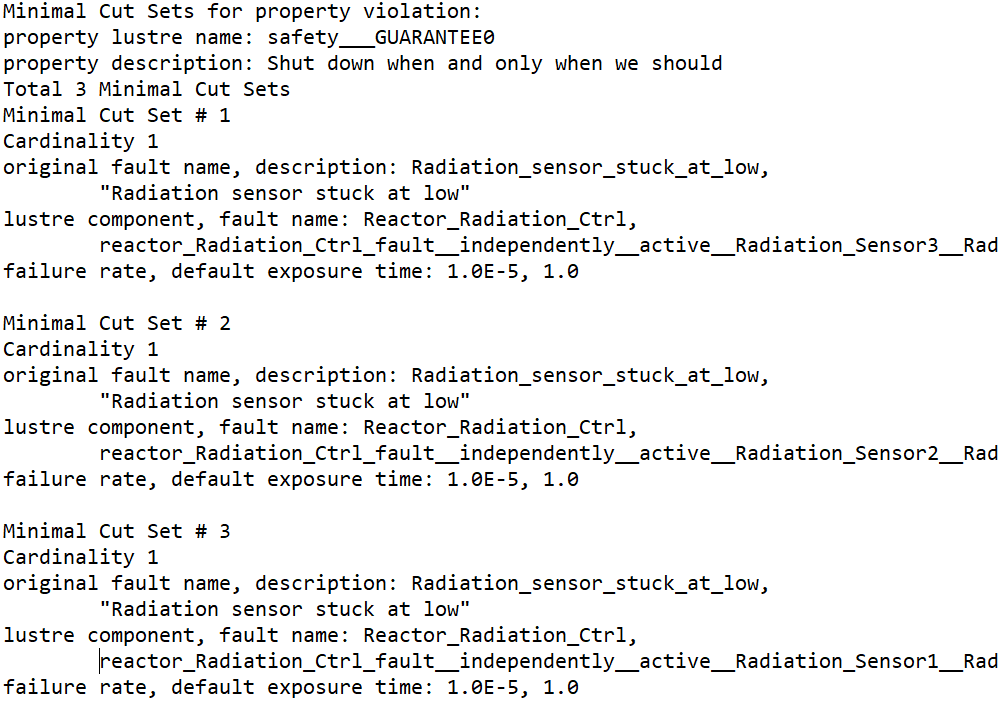
\includegraphics[scale=0.7]{images/detailedMCS.png}
	\caption{Detailed Output of MinCutSets}
		\label{fig:detailedMCS}
	\end{center}
\end{figure}

\item The minimal cut set information can be presented in tally form. This does not contain the fault information in detail, but instead gives only the tally of cut sets per property. This is useful in large models with many cut sets as it reduces the size of the text file. An example of this output type is seen in Figure~\ref{fig:tallyMCS}.
\begin{figure}[h!]
	\hspace*{-2cm}
	\vspace{-0.1in} 
	\begin{center}
		\includegraphics[scale=0.7]{images/TallyMCS.png}
	\caption{Tally Output of MinCutSets}
		\label{fig:tallyMCS}
	\end{center}
\end{figure}

\item The tool can also generate fault tree and minimal cut set information formatted as input to the SOTERIA tool~\cite{manolios2019model} to produce hierarchical fault trees that are consistent with the system architecture/component verification layers, or flat fault trees consist of minimal cut sets only, both in graphical form. A sample graphical fault tree output from the SOTERIA tool is shown in Figure~\ref{fig:soteriaFT}. The SOTERIA tool is also able to compute the probabilities for the top level event from a given fault tree. However, based on experience with the WBS example, our tool was a more scalable solution as it produces minimal cut sets for more complex systems, also in shorter amount of time. The text format of the minimal cut sets seemed anectodally easier to read than the graphical format for larger systems. 
% minimal cut set information can also be formatted as input to the SOTERIA tool \janet{[new soteria reference]} to display. 
%This
%\janet{The SOTERIA} tool can \janet{produce fault trees in }
%use the auto generated ocaml file to produce optimized fault trees in a graphical format instead of textual format. (See Section on SOTERIA for more information.) A sample output is shown in Figure~\ref{fig:soteriaMCS}. This \textit{.ml} file can be given as input to %SOTERIA to produce the optimized fault tree shown in Figure~\ref{fig:}. 
\begin{comment}
\begin{figure}[h!]
	\hspace*{-2cm}
	\vspace{-0.1in} 
	\begin{center}
		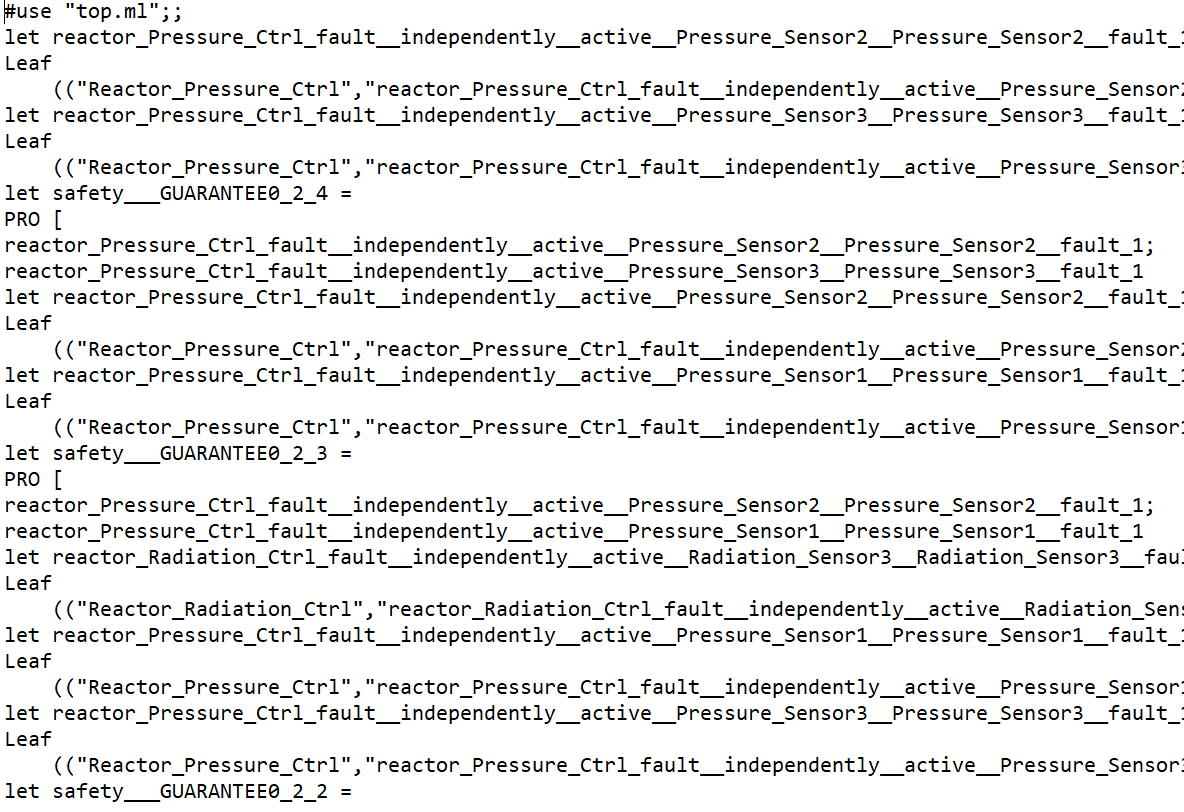
\includegraphics[scale=0.5]{images/soteriaMCS.png}
	\caption{SOTERIA Output of MinCutSets}
		\label{fig:soteriaMCS}
	\end{center}
\end{figure}
\end{comment}

\begin{figure}[h!]
	\hspace*{-2cm}
	\vspace{-0.1in} 
	\begin{center}
		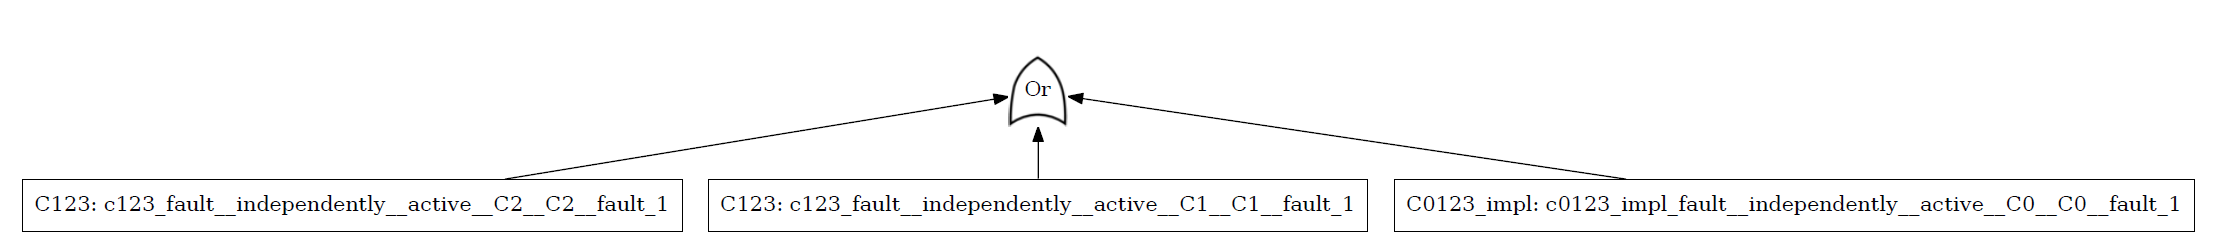
\includegraphics[scale=0.25]{images/Soteria_FT.png}
		\caption{Example SOTERIA Fault Tree}
		\label{fig:soteriaFT}
	\end{center}
\end{figure}

\end{enumerate}

\subsubsection{Use of Analysis Results to Drive Design Change}
We use a single top level requirement of the WBS: S18-WBS-0323 (Never indadvertent braking with all wheels locked to illustrate how Safety Annex can be used to detect design flaws and how faults can affect the behavior of the system). This safety property description can be found in detail in Section \ref{sec:fault_modeling}. Upon running max $n$ compositional fault analysis with $n = 1$, this particular fault was shown to be a single point of failure for this safety property. A counterexample is shown in Figure \ref{fig:counterexample} showing the active fault on the pedal sensor. 

\begin{figure}[h!]
	%\vspace{-0.2in}
	\begin{center}
		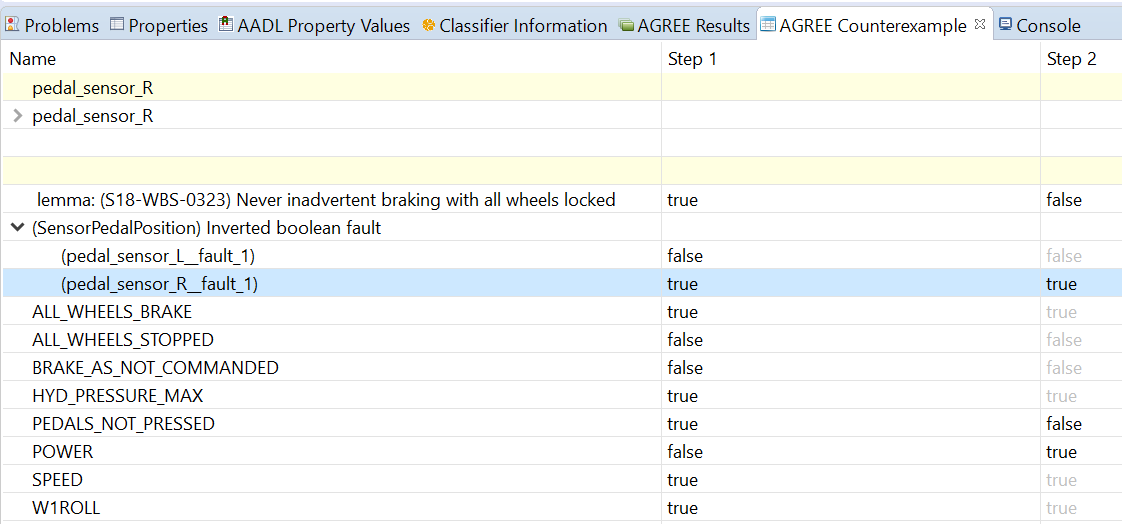
\includegraphics[width=\textwidth]{images/counterexample.png}
	\end{center}
	\vspace{-0.3in}
	\caption{AGREE counterexample for inadvertent braking safety property}
	\label{fig:counterexample}
	%\vspace{-0.2in}
\end{figure} 

Depending on the goals of the system, the architecture currently modeled, and the mitigation strategies that are desired, various strategies are possible to mitigate the problem.

\begin{itemize}
\item Possible mitigation strategy 1: Monitor system can be added for the sensor: A monitor sub-component can be modeled in which it accesses the mechanical pedal as well as the signal from the sensor. If the monitor finds discrepancies between these values, it can send an indication of invalid sensor value to the top level of the system. In terms of the modeling, this would require a change to the behavioral contracts which use the sensor value. This validity would be taken into account through the means of $valid \land pedal\_sensor\_value$. 
%In the real system however, this mitigation would need to be taken into account. Whether this is a flag to the pilot who can then override the electrical system and switch to a different mode or perform some other action to mitigate the failed sensor must be discussed and implemented. 

\item Possible mitigation strategy 2: Redundancy can be added to the sensor: A sensor subsystem can be modeled which contains 3 or more sensors. The overall output from the sensor system may utilize a voting scheme to determine validity of sensor reading. There are multiple voting schemes that are possible, one of which is a majority voting (e.g. one sensor fails, the other two take majority vote and the correct value is passed). 
When three sensors are present, this mitigates the single point of failure problem. New behavioral contracts are added to the sensor system to model the behavior of redundancy and voting. 
\end{itemize}

In the case of the pedal sensor in the WBS, the latter of the two strategies outlined above was implemented. A sensor system was added to the model which held three pedal sensors. The output of this subsystem was constrained using a majority voting scheme. Upon subsequent runs of the analysis (regardless which type of run was used), resilience was confirmed in the system regarding the failure of a single pedal sensor. Figure \ref{fig:sensorsystem} outlines these architectural changes that were made in the model.

\begin{figure}[h!]
	%\vspace{-0.2in}
	\begin{center}
		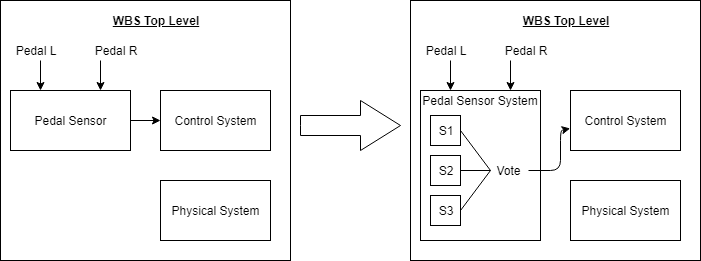
\includegraphics[width=\textwidth]{images/sensorsystem.png}
	\end{center}
	\vspace{-0.3in}
	\caption{Changes in the architectural model for fault mitigation}
	\label{fig:sensorsystem}
	%\vspace{-0.2in}
\end{figure}

As can be seen through this single example, a system as large as the WBS would benefit from many iterations of this process. Furthermore, if the model is changed even slightly on the system development side, it would automatically be seen from the safety analysis perspective and any negative outcomes would be shown upon subsequent analysis runs. This effectively eliminates any miscommunications between the system development and analysis teams and creates a new safeguard regarding model changes. 

For more information on types of fault models that can be created as well as details on analysis results, see the users guide located in the GitHub repository \cite{SAGithub}. This repository also contains all models used in this project. 




\section{Related Work}
\label{sec:related_work}

A model-based approach for safety analysis was proposed by Joshi et. al in \cite{Joshi05:Dasc, Joshi05:SafeComp, Joshi07:Hase}.  In this approach, a safety analysis system model (SASM) is the central artifact in the safety analysis process, and traditional safety analysis artifacts, such as fault trees, are automatically generated by tools that analyze the SASM.

The contents and structure of the SASM differ significantly across different conceptions of MBSA.  We can draw distinctions between approaches along several different axes.  The first is whether they propagate faults explicitly through user-defined propagations, which we call {\em failure logic modeling} (FLM) or through existing behavioral modeling, which we call {\em failure effect modeling} (FEM).  The next is whether models and notations are {\em purpose-built} for safety analysis vs. those that extend {\em existing system models} (ESM).

For FEM approaches, there are several additional dimensions.  One dimension involves whether {\em causal} or {\em non-causal} models are allowed.  Non-causal models allow simultaneous (in time) bi-directional %failure
error propagations, which allow more natural expression of some failure types (e.g. reverse flow within segments of a pipe), but are more difficult to analyze.  A final dimension involves whether analysis is {\em compositional} across layers of hierarchically-composed systems or {\em monolithic}.  Our approach is an extension of AADL (ESM), causal, compositional, mixed FLM/FEM approach.

%We believe this is in a unique area of the trade space compared to other state-of-the-art MBSA approaches.

%Formal model based systems engineering (MBSE) methods and tools now permit system level requirements to be specified and analyzed early in the development process~\cite{QFCS15:backes,CIMATTI2015333, NFM2012:CoGaMiWhLaLu, hilt2013:MuWhRaHe}. Design models from which aircraft systems are developed can be integrated into the safety analysis process to help guarantee accurate and consistent results. Integration of MBSA into safety analysis process is described by Bozzano and Villafiorita~\cite{Bozzano:2010:DSA:1951720}. There are tools that currently support reasoning about faults in architecture description languages such as SysML and AADL. We provide here a brief overview of the most relevant safety analysis tools.

%In analyzing an EMV2 model of the WBS, we found missing feedback loops between the wheels and BSCU
%Interactions are easily overlooked by analysts and thus not explicitly described. In our approach, faults are injected into the system and behaviorally propagated through the use of assume-guarantee statements in AGREE. This avoids the difficulties inherent with explicit fault enumeration and propagation.

Tools such as the AADL Error Model Annex, Version 2 (EMV2)~\cite{EMV2} and HiP-HOPS for EAST-ADL~\cite{CHEN201391} are {\em FLM}-based {\em ESM} approaches.  As previously discussed, given many possible faults, these propagation relationships require substantial user effort and become more complex.  In addition, it becomes the analyst's responsibility to determine whether faults can propagate; missing propagations lead to unsound analyses.  In our Safety Annex, propagations occur through system behaviors (defined by the nominal contracts) with no additional user effort.

The model-based safety assessment toolset COMPASS (Correctness, Modeling project and Performance of Aerospace Systems)~\cite{10.1007/978-3-642-04468-7_15} is closely related to our work.  COMPASS is a mixed {\em FLM/FEM}-based, {\em causal} {\em compositional} tool suite that uses the SLIM language, which is based on a subset of AADL, for its input models~\cite{5185388, criticalembeddedsystems}. In SLIM, a nominal system model and the error model are developed separately and then transformed into an extended system model.  This extended model is automatically translated into input models for the NuSMV model checker~\cite{Cimatti2000, NuSMV}, MRMC (Markov Reward Model Checker)~\cite{Katoen:2005:MRM:1114692.1115230, MRMC}, and RAT (Requirements Analysis Tool)~\cite{RAT}. The safety analysis tool xSAP~\cite{DBLP:conf/tacas/BittnerBCCGGMMZ16} can be invoked in order to generate safety analysis artifacts such as fault trees and FMEA tables~\cite{compass30toolset}.  COMPASS is an impressive tool suite, but some of the features that make AADL suitable for SW/HW architecture specification: event and event-data ports, properties, threads, and processes, appear to be missing, which means that the SLIM language may not be suitable as a general system design notation (ESM). A SLIM nominal model is extended by creating an error model. This is defined by type, implementation, and effect. Furthermore, the error model specifies outgoing and incoming propagations similar to the EMV2 error annex for AADL\cite{EMV2}. Outgoing error propagations report the error state to other components. If their error states are affected, the other components will have a corresponding incoming propagation~\cite{10.1007/978-3-642-04468-7_15,compass30toolset,COMPASSusersguide}. This differs from our approach in that error propagations do not need to be specified and the propagations are performed behaviorally through the violation of contracts on connected components.

%While it is clear that behavioral contracts can be specified in the SLIM model through the use of assume-guarantee statements, the focus of the tool and examples provided is on explicit fault propagation much like EMV2 AADL error annex~\cite{COMPASSusersguide}. Our approach is different in that the focus is not on explicit fault propagation, but instead leveraging the nominal model behavior in order to view the system behavior in the presence of faults.


% Say something about behavioral propagation here ---------------------------------------------------

SmartIFlow~\cite{info8010007} is a {\em FEM}-based, {\em purpose-built}, {\em monolithic} {\em non-causal} safety analysis tool that describes components and their interactions using finite state machines and events. Verification is done through an explicit state model checker which returns sets of counterexamples for safety requirements in the presence of failures.  SmartIFlow allows {\em non-causal} models containing simultaneous (in time) bi-directional %failure
error propagations.  On the other hand, the tools do not yet appear to scale to industrial-sized problems, as mentioned by the authors~\cite{info8010007}: ``As current experience is based on models with limited size, there is still a long way to go to make this approach ready for application in an industrial context''.


The Safety Analysis and Modeling Language (SAML)~\cite{Gudemann:2010:FQQ:1909626.1909813} is a {\em FEM}-based, {\em purpose-built}, {\em monolithic} {\em causal} safety analysis language.  System models constructed in SAML can be used used for both qualitative and quantitative analyses. It allows for the combination of discrete probability distributions and non-determinism. The SAML model can be automatically imported into several analysis tools like NuSMV~\cite{Cimatti2000}, PRISM (Probabilistic Symbolic Model Checker)~\cite{CAV2011:KwNoPa}, or the MRMC probabilistic model checker~\cite{Katoen:2005:MRM:1114692.1115230}. 
%The focus of SAML is to provide modeling support for safety analysis. This is a different focus than what the safety annex provides through AADL.

%Given that AADL is an SAE International standard modeling language, the goal of AADL is system engineering and the development of performance-critical, embedded, real-time systems. What we accomplish is to provide safety engineers with a way to incorporate safety engineering into already existing model development practices in industry.

%In earlier work, an approach to MBSA was demonstrated using the Simulink\textsuperscript{\textregistered} notation~\cite{Joshi05:SafeComp,Joshi05:Dasc}. In this approach, a behavioral model of system dynamics was used to reason about the effects of faults in the system. This approach allows an implicit and natural notion of fault propagation through the system. However, non-functional architectural properties were not captured as Simulink is not designed as an architecture description language. In our approach, we are applying quantitative reasoning and implicit fault propagation to a more rich architecture language.

AltaRica~\cite{PROSVIRNOVA2013127,BieberERTS2018} is a {\em FEM}-based, {\em purpose-built}, {\em monolithic} safety analysis language with several dialects.  There is one dialect of AltaRica which use dataflow ({\em causal}) semantics, while the most recent language update (AltaRica 3.0) uses non-causal semantics.  The dataflow dialect has substantial tool support, including the commercial Cecilia OCAS tool from Dassault~\cite{bieber2004safety}.  For this dialect the Safety assessment, fault tree generation, and functional verification can be performed with the aid of NuSMV model checking~\cite{symbAltaRica}. Failure states are defined throughout the system and flow variables are updated through the use of assertions~\cite{Bieber04safetyassessment}.  AltaRica 3.0 has support for simulation and Markov model generation through the OpenAltaRica (www.openaltarica.fr) tool suite.

Formal verification tools based on model checking have been used to automate the generation of safety artifacts~\cite{symbAltaRica,10.1007/978-3-540-75596-8-13, DBLP:conf/tacas/BittnerBCCGGMMZ16}. This approach has limitations in terms of scalability and readability of the fault trees generated. Work has been done towards mitigating these limitations by the scalable generation of readable fault trees~\cite{10.1007/978-3-319-11936-6-7}.






\section{Conclusion}


We have developed an extension to the AADL language with tool support for formal analysis of system safety properties in the presence of faults. Faulty behavior is specified as an extension of the nominal model, allowing safety analysis and system implementation to be driven from a single common model. Both symmetric and asymmetric faulty behaviors are supported. This new Safety Annex leverages the AADL structural model and nominal behavioral specification (using the AGREE annex) to propagate faulty component behaviors without the need to add separate propagation specifications to the model. Implicit %failure
error propagation enables safety engineers to inject failures/faults at component level and assess the effect of behavioral propagation at the system level. It also supports explicit 
%failure
error propagation that allows safety engineers to describe dependent faults that are not easily captured using implicit %failure
error propagation. Generation of minimal cut sets collects all minimal set of fault combinations that can cause violation of the top level properties. 
%\danielle{Next steps will include applying and assessing the approach in safety assessment of avionics products, and enhance the usability of the analysis results.} 
For more details on the tool, models, and approach, see the Architectural Modeling and Analysis for Safety Engineering (AMASE) project final report for NASA~\cite{AMASEFinalReport}. 
To access the tool plugin, users manual, or models, see the repository~\cite{SAGithub}. 

%The Safety Annex allows both implicit and explicit failure propagation. This enables safety engineers to inject failures/faults at component level and assess the effect of behavioral propagation at the system level as well as describe dependent faults that are not easily captured using implicit failure propagation. The toolset (AADL, AGREE, and Safety Annex) describes the nominal model (absence of faults) and the faulty model in a cleanly separated and yet analyzable fashion. This serves to preserve the system model for the systems engineering process and simultaneously be able to see their combined effect on the system behavior. 

\vspace{2 mm}
\noindent {\bf Acknowledgments.} This research was funded by NASA contract NNL16AB07T and the University of Minnesota College of Science and Engineering Graduate Fellowship.


\balance
%\noindent {\bf Acknowledgments.} This research was funded by NASA contract NNL16AB07T and the University of Minnesota College of Science and Engineering Graduate Fellowship.

%\vspace{-0.40cm}
\bibliographystyle{abbrv}
\bibliography{biblio2}
%\vspace{-7.25cm}
% This ~ seems to fix an odd bibliography alignment issue
%~

%\ifdefined\TECHREPORT
%\appendix
%
%\section{Appendix: Proof of Equivalence}
%\input{appendix}
%\fi

%\section{Appendix: GPCA CENTA Model}
%\label{appendix:gpcacenta}
%\begin{figure}[!ht]
%\begin{center}
%\includegraphics[scale=0.6]{images/sampled_pca.PNG} %[trim = 0 2 0 0, clip=true]{Comp}
%\caption{GPCA AGREE Properties modeled as a Timed Automata} \label{fig:samplepca}
%\end{center}
%\end{figure}

%\balancecolumns

\end{document} 